% ===========================================================================
% DAS732 A3 team report.  Compile from the report/ folder:
%     pdflatex main.tex  &&  pdflatex main.tex      (run twice for references)
% Overleaf: upload the whole repository (or at least report/, images/ and
% reference/DV_Assignment1_report.pdf) and set main.tex as the main document.
%
% Status of each section
%   01_introduction.tex      Advaya  (TODO)
%   02_data_handling.tex     Tushaar (DONE)
%   03_workflow.tex          Tushaar (DONE; diagram rows for M2/M3 to update)
%   04_member1_tushaar.tex   Tushaar (DONE)
%   05_member2_advaya.tex    Advaya  (TODO, structure provided)
%   06_member3_aman.tex      Aman    (TODO, structure provided)
%   07_synthesis.tex         Advaya + Aman (TODO, Tushaar's input provided)
%   08_conclusions.tex       Advaya  (TODO)
%   09_contributions.tex     all     (Tushaar row DONE)
%   11_references.tex        all     (Tushaar references DONE; add yours)
% Delete \todo{...} boxes as you fill sections. Search "TODO" to find them.
% ===========================================================================
\documentclass[11pt]{article}
\usepackage[a4paper,margin=2.2cm]{geometry}
\usepackage[T1]{fontenc}
\usepackage{lmodern}
\usepackage{booktabs,graphicx,amsmath,amssymb,float,rotating,pdfpages,xcolor}
\usepackage[hidelinks]{hyperref}
\graphicspath{{../}}   % image paths in the sections are relative to the repo root

% Red TODO box: remove each one once its content is written.
\newcommand{\todo}[1]{\leavevmode\par\noindent\fcolorbox{red}{red!5}{\parbox{\dimexpr\linewidth-2\fboxsep-2\fboxrule}{\color{red!70!black}\textbf{TODO: }#1}}\par\medskip}

% Inline red TODO for use inside captions.
\DeclareRobustCommand{\todoi}[1]{{\color{red!70!black}\textbf{TODO:} #1}}

% \teamfig{width}{path}{caption}{label}: includes the image if it exists,
% otherwise draws a placeholder so the report always compiles.
\newcommand{\teamfig}[4]{%
  \begin{figure}[htbp]\centering
  \IfFileExists{../#2}{\includegraphics[width=#1]{#2}}%
    {\fcolorbox{red}{red!5}{\parbox[c][4cm][c]{0.8\linewidth}{\centering\color{red!70!black}missing image: \texttt{\detokenize{#2}}}}}%
  \caption{#3}\label{#4}\end{figure}}

\title{\textbf{Visual Analytics of Student Habits, Wellbeing and Performance}\\[4pt]
\large DAS732 Data Visualization: Programming Assignment A3}
\author{Kolipakula Sai Tushaar (BT2024022) \and Advaya Bhardwaj (BT2024231) \and Aman Kumar Lahoti (BT2024123)}
\date{November 2026}

\begin{document}
\maketitle
\tableofcontents
\clearpage

% ---------------------------------------------------------------------------
% OWNER: Advaya.  Replace the TODO box with ~half a page. Keep it plain.
% ---------------------------------------------------------------------------
\section{Introduction}
\label{sec:intro}

\todo{Write about half a page covering:
(1) the dataset in one sentence (80{,}000 students, habits, wellbeing,
background, prior GPA, exam score);
(2) what A1 found, in two sentences: prior GPA correlates $r=0.93$ with the exam
score and the apparent effects of habits and wellbeing collapse once it is
controlled; the score is capped at 100;
(3) the A3 question: \emph{what do habits, wellbeing and background add to
our understanding of performance once prior attainment, redundant measures
and score ceilings are accounted for?};
(4) how A3 answers it: one shared preprocessing stage, three strands
(clustering, classification, regression), each with a feedback loop
(Section~\ref{sec:workflow});
(5) one sentence pointing to the A1 report in the Appendix.}

% ---------------------------------------------------------------------------
% Shared section: A3 data handling (written by Kolipakula Sai Tushaar).
% DONE - no edits needed. Compiled through report/main.tex.
% ---------------------------------------------------------------------------
\section{A3 Data Handling}
\label{sec:a3-prep}

A3 starts from \texttt{master\_cleaned.csv}, the output of the A1 pipeline
(80{,}000 rows, 43 columns, no nulls or duplicates; see the A1 report in the Appendix). The script
\texttt{preprocess\_a3.py} adds eight steps that the A3 models need and that A1
did not. Every step asserts its own precondition, so the script fails loudly
if the input ever changes. It writes one shared table, \texttt{a3\_base.csv.gz},
which all three members load through \texttt{a3\_common.load\_base()} so that
every analysis uses the same features, split and colours.

\begin{enumerate}
  \item \textbf{Re-validation.} Schema, null, duplicate and range checks on 14
        numeric columns are repeated before any modelling.
  \item \textbf{Exact redundancies removed.} Three columns are formulas of
        others for every row and would double-weight one variable in a
        distance-based or linear model:
        \begin{itemize}
          \item \texttt{exam\_anxiety\_score} $=\mathrm{clip}(15-\text{motivation},5,10)$;
          \item \texttt{study\_hours\_per\_week} $=7\times$ daily study hours;
          \item \texttt{leisure\_screen\_hours} $=$ social media $+$ streaming hours.
        \end{itemize}
  \item \textbf{Leakage recorded.} \texttt{dropout\_risk} equals
        $(\text{stress}>8)\wedge(\text{motivation}\le 3)$ for all rows
        (A1 report, Fig.~21), and \texttt{performance\_band} and
        \texttt{performance\_delta} are functions of the exam score. These
        rules are stored in \texttt{a3\_feature\_groups.json} so no model uses
        them as features by mistake.
  \item \textbf{Ceiling flags.} 25.8\% of students score exactly 100 and
        40.0\% have a prior GPA of exactly 4.0; 21.4\% are at both caps. Both
        variables are censored, which matters for any residual or linear model.
  \item \textbf{Prior-attainment bands.} \texttt{gpa\_band} on
        \texttt{previous\_gpa\_pct}: Below 80 (17{,}487 students, mean score
        71.7), 80--90 (15{,}154; 85.2), 90--99 (15{,}390; 94.4) and Elite, GPA
        exactly 4.0 (31{,}969; 98.0).
  \item \textbf{Outlier screen.} The $1.5\times$IQR rule flags 0.25--0.45\% of
        values in five columns. All lie inside the instrument ranges, so they
        are kept as genuine tail values.
  \item \textbf{Encoding.} Booleans become 0/1; four nominal columns (gender,
        major, study environment, learning style) become 18 one-hot columns;
        ordinal columns keep their A1 integer codes.
  \item \textbf{Train/test split.} 80/20, stratified on performance band
        $\times$ dropout flag, seed 42. Train: 64{,}000 rows, mean score 89.13,
        dropout rate 1.98\%; test: 16{,}000 rows, 89.19, 1.98\%.
\end{enumerate}

\paragraph{Supplementary data.} None is used. Every question in A3 can be
answered from the A1 dataset itself, and the strongest explanatory variable,
prior GPA, is already in it. The VAST 2026 Challenge material mentioned in the
brief was not used.

Scaling is deliberately left out of the shared file. Each member fits the
scaler on the training split inside their own pipeline, so no information from
the test split reaches any model.

\section{Visual analytics workflow}
\label{sec:workflow}

Figure~\ref{fig:master-workflow} follows the visual analytics process of
Keim et~al.~\cite{keim2008}. Following a strand shows what data went
into a model, what the analyst inspected, and which observation motivated a
change. The edge labelled \emph{Feedback loop} connects the first
inference to the transformation. The second set of models and views then
shows what changed.

The three analysts use the fixed split from Section~\ref{sec:a3-prep} for
different questions. Tushaar clusters students by their habits, checks how
the clusters differ in prior attainment and exam scores, then fits fresh
models within each prior-GPA band. Advaya's classification strand examines
how well the dropout flag can be recovered after removing the inputs that
define it. Aman's regression strand examines how the score ceiling and
prior attainment change the interpretation of background variables and
tutoring. The common identifiers, outcome definitions and split allow the
team to compare these findings.

\begin{figure}[H]
  \centering
  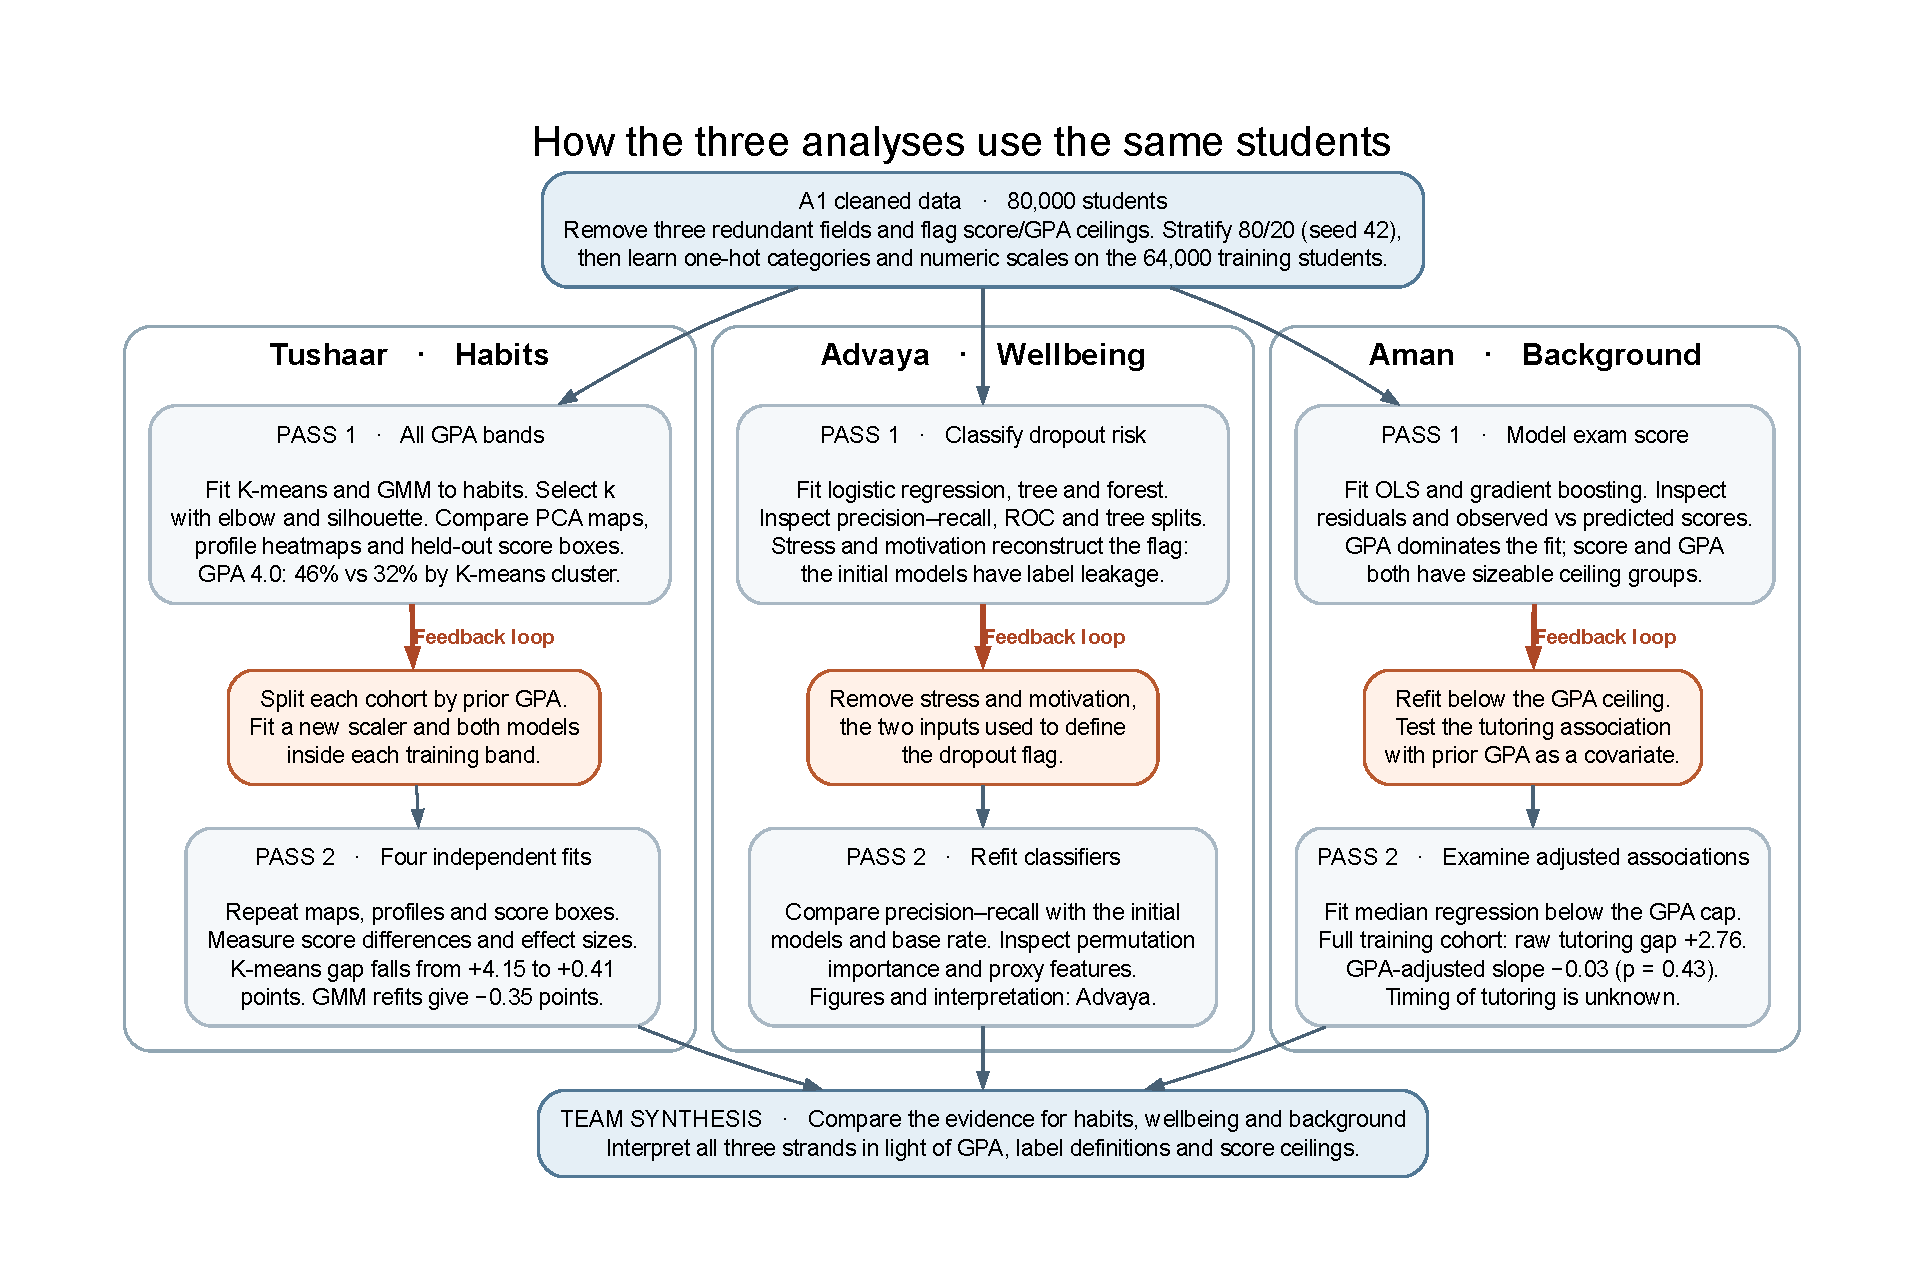
\includegraphics[width=\textwidth,height=.37\textheight,keepaspectratio]{diagrams/A3_master_workflow.pdf}
  \caption{The shared A3 workflow. Each column unrolls one analyst's two
  iterations. The labelled edge records the inference that changes the
  next analysis.}
  \label{fig:master-workflow}
\end{figure}

\clearpage
% ---------------------------------------------------------------------------
% Member 1 section: Kolipakula Sai Tushaar - what students do.
% DONE - no edits needed. Every number below is produced by
% Member1/m1_clustering_workflow.py and stored in Member1/outputs/m1_results.json.
% ---------------------------------------------------------------------------
\section{Kolipakula Sai Tushaar: Habit Profiles (Clustering)}
\label{sec:m1}

\paragraph{Driving question.} A1 (Appendix, Figs.~1--11) showed that study hours, sleep,
exercise and the leisure share of screen time each move the exam score by a few
points. A3 asks the next question: \emph{do students form distinct habit
profiles, and does belonging to a ``good-habits'' profile give an exam
advantage beyond the student's prior attainment?} Clustering is the right tool
because it groups students by their whole habit pattern without being told the
outcome; the outcome is only used afterwards to judge the groups.

\paragraph{Method summary.} K-means~\cite{lloyd1982} on standardised features
(scaler fitted on the training split, scikit-learn~\cite{pedregosa2011}), with the number of clusters $k$ chosen from four
diagnostics: the elbow in inertia, the silhouette~\cite{rousseeuw1987} compared against a
\emph{shuffled null} (each column permuted independently, which keeps every
variable's distribution but destroys any joint structure), seed stability
(mean adjusted Rand index~\cite{hubert1985} between six single-start runs) and Gaussian-mixture
BIC. The Hopkins statistic~\cite{hopkins1954} is reported as a supporting check.
Cluster differences in score are tested with Kruskal--Wallis~\cite{kruskal1952} and
$\eta^2_H$ (iteration~1), and with Welch's $t$~\cite{welch1947}, Mann--Whitney
$U$~\cite{mann1947}, Cohen's $d$~\cite{cohen1988} and 1{,}000-sample bootstrap
confidence intervals~\cite{efron1993} (iteration~2). A gradient-boosting
regressor~\cite{friedman2001} with permutation importance~\cite{breiman2001}
cross-checks the clustering result. Iteration~2 is
confirmed on the 16{,}000-student test split, which no model or adjustment
ever saw. Fig.~\ref{fig:m1-workflow} shows the full workflow.

\begin{sidewaysfigure}
  \centering
  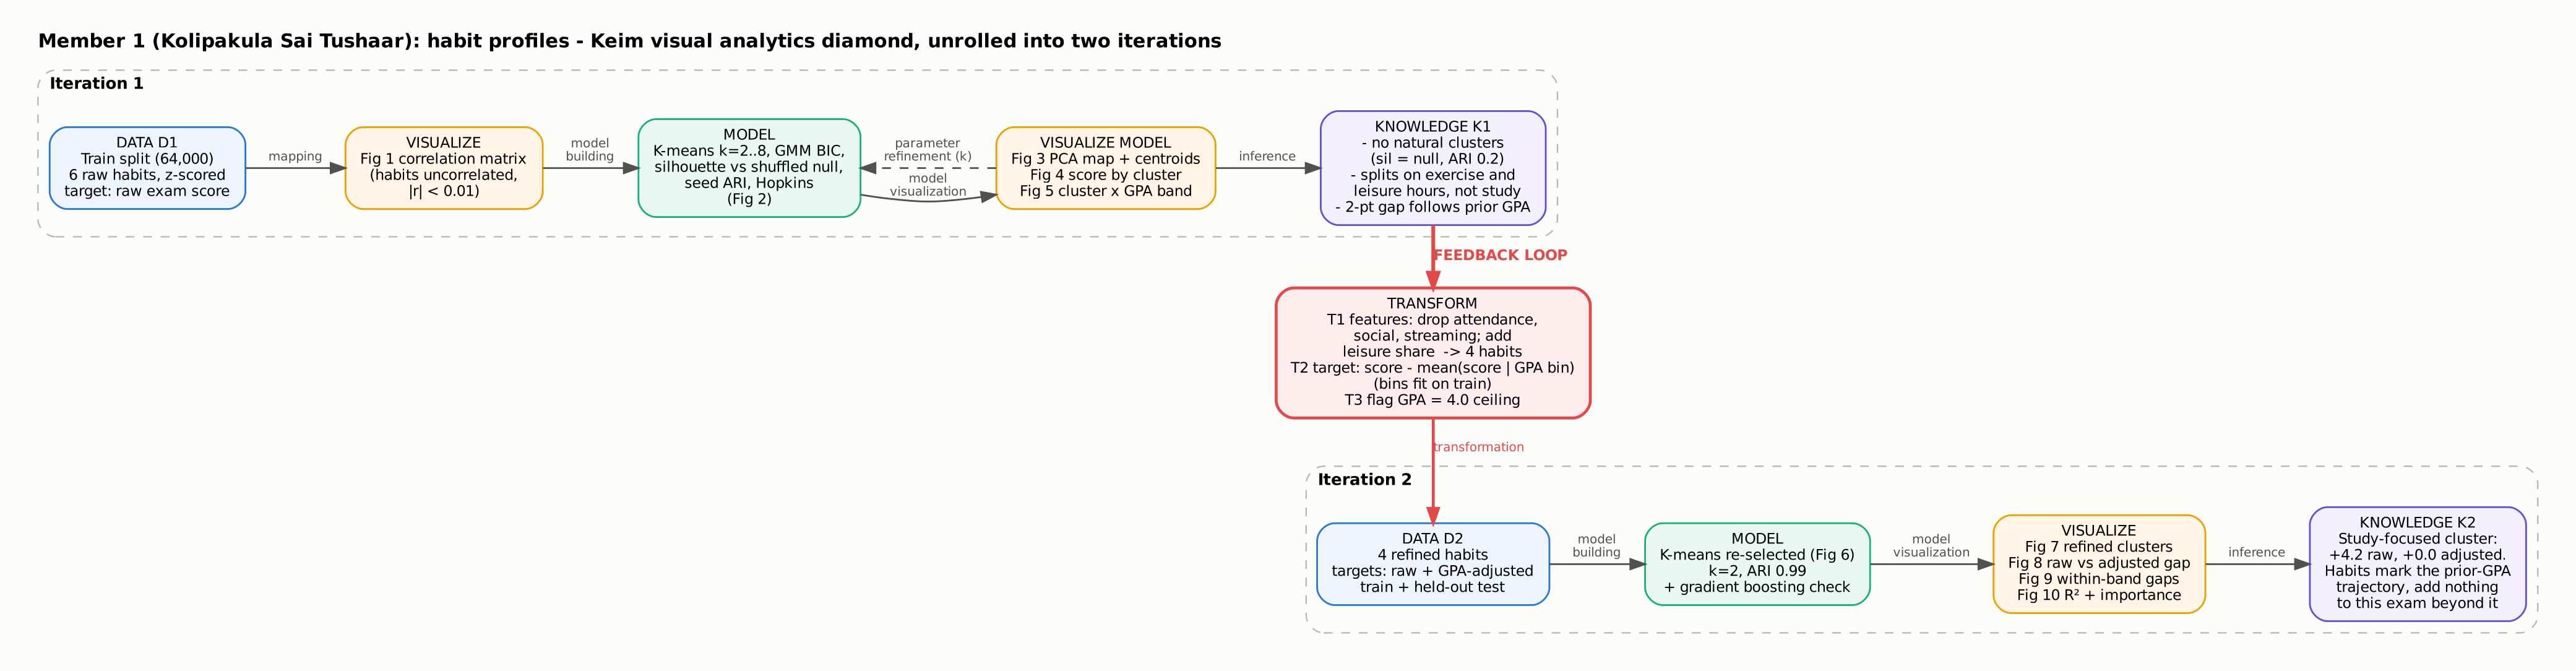
\includegraphics[width=\textheight]{images/M1_workflow_unrolled.png}
  \caption{Member~1's workflow as the Keim et~al.\ diamond unrolled into two
  iterations. The only self-loop is the parameter refinement of $k$ inside
  iteration~1. The edge labelled \emph{Feedback loop} carries the iteration-1
  inference into three data transformations (T1--T3) that define the data for
  iteration~2.}
  \label{fig:m1-workflow}
\end{sidewaysfigure}

\begin{table}[htbp]
  \centering\small
  \caption{Task sequence and the reason behind each visualization.}
  \label{tab:m1-tasks}
  \begin{tabular}{@{}lllp{10.4cm}@{}}
    \toprule
    Stage & Fig. & Task & Why this chart \\
    \midrule
    V1 & \ref{fig:m1-corr} & Correlate & A matrix shows every pair at once; any joint structure clustering could find must show up here first. \\
    M1 & \ref{fig:m1-k1} & Select $k$ & Four small multiples on one $k$ axis; the dashed null line makes ``better than random'' visible. \\
    V1 & \ref{fig:m1-map1} & Overview & Hexbin density (80k points would overplot); clusters faceted, not overlaid, because four hues on one scatter are not colour-blind safe. Heatmap gives the profile. \\
    V1 & \ref{fig:m1-score1} & Compare & Violins show the overlap; means with CIs show the size of the gap on a readable scale. \\
    V1 & \ref{fig:m1-conf1} & Explain & 100\% stacked bars for composition; dot plot within each band to test the confound. \\
    M2 & \ref{fig:m1-k2} & Re-select $k$ & Same panels as Fig.~\ref{fig:m1-k1} with D1 in grey, so the change is the only new information. \\
    V2 & \ref{fig:m1-map2} & Overview & With two clusters a direct scatter is legible; diverging bars give centroids in $z$ with raw-unit labels. \\
    V2 & \ref{fig:m1-gap} & Compare & One axis (points) for raw, adjusted and GPA gaps, so the reader compares lengths directly. \\
    V2 & \ref{fig:m1-band} & Search & Raw and adjusted gap side by side per band locates where any gap survives. \\
    M2/V2 & \ref{fig:m1-sup} & Validate & A supervised model confirms the clustering conclusion with a different method. \\
    \bottomrule
  \end{tabular}
\end{table}

% ---------------------------------------------------------------------------
\subsection{Iteration 1: clustering the six raw habits}

\paragraph{Data D1.} Six raw, non-derived habit variables from the training
split: daily study hours, sleep hours, weekly exercise, attendance, social
media hours and streaming hours. Derived columns are left out so that no
behaviour is counted twice.

\begin{figure}[htbp]
  \centering
  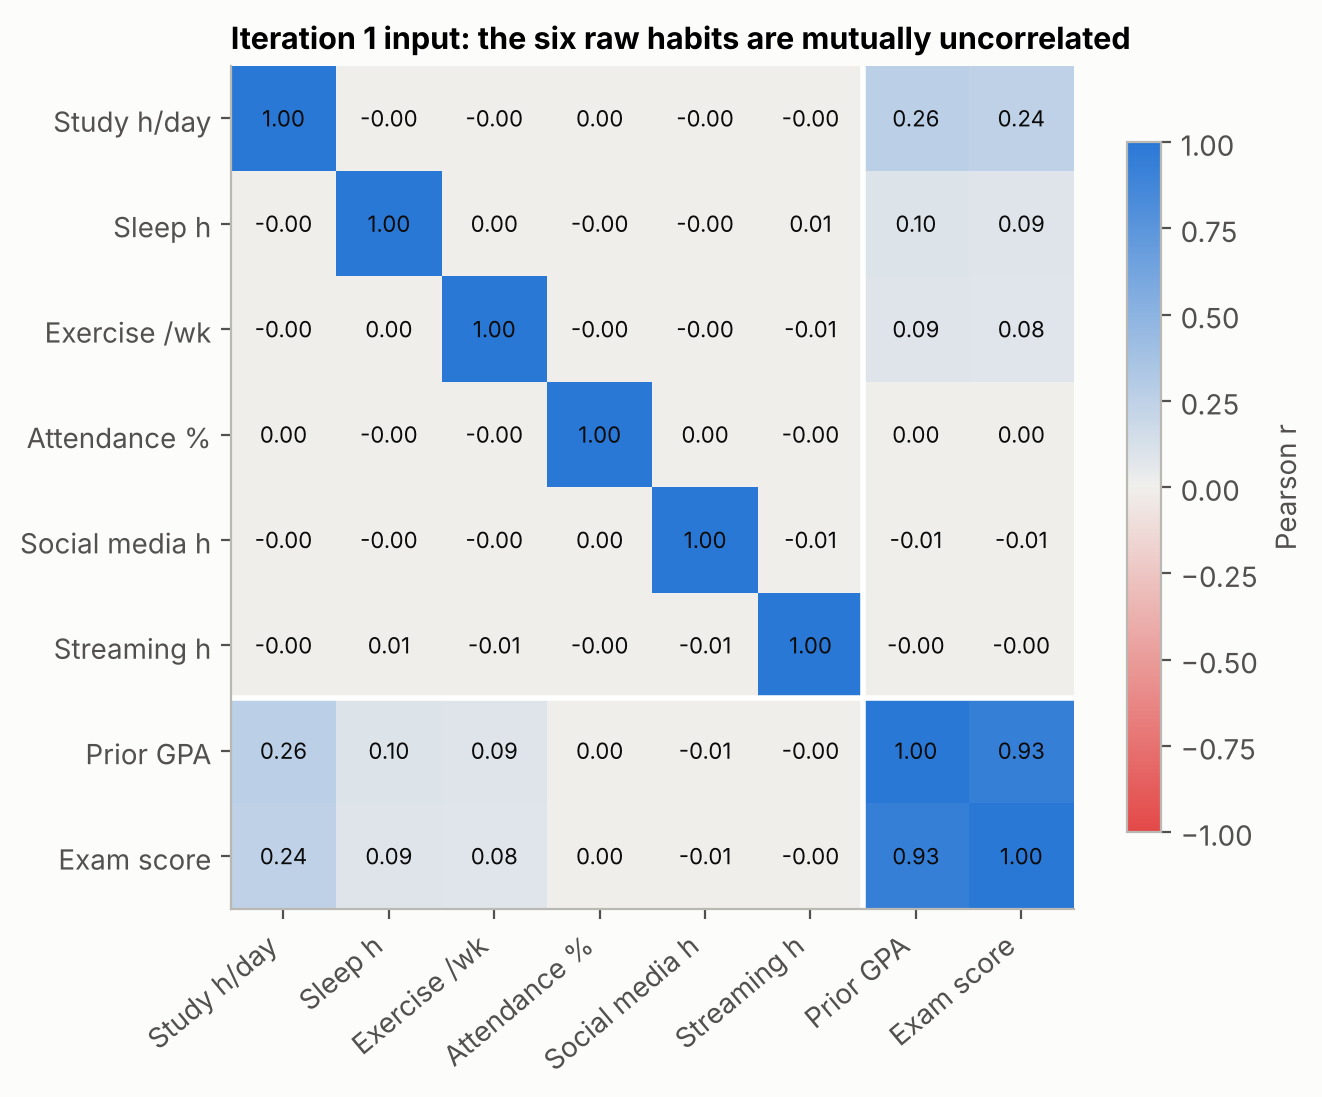
\includegraphics[width=0.62\textwidth]{images/M1_fig01_habit_correlations.png}
  \caption{Pearson correlations among the six habits, prior GPA and exam score
  (training split). Off the diagonal, no pair of habits correlates above
  $|r|=0.007$. Only study hours ($r=0.24$), sleep (0.09) and exercise (0.09)
  relate to the exam score, and each relates almost equally to prior GPA.}
  \label{fig:m1-corr}
\end{figure}

Fig.~\ref{fig:m1-corr} is the first warning. The six habits are statistically
independent of each other, so the habit space has no obvious joint structure
for clustering to find. Attendance, social media and streaming hours have no
correlation with the score at all ($|r|\le 0.006$).

\begin{figure}[htbp]
  \centering
  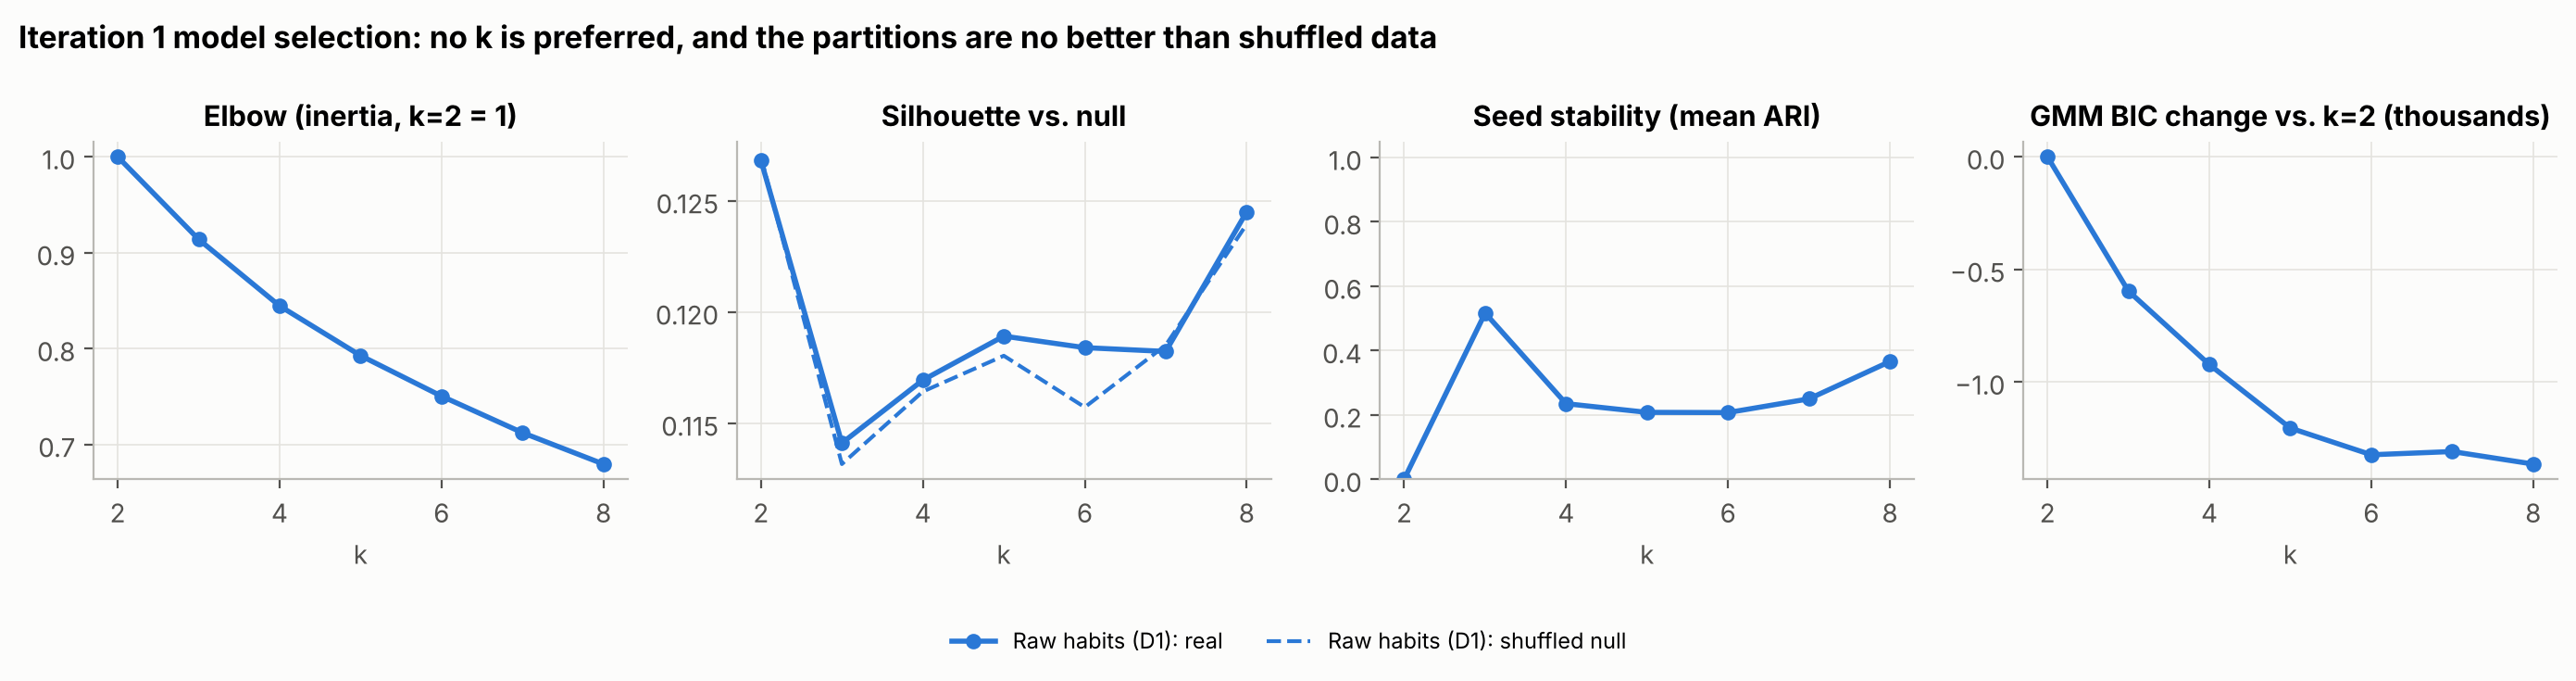
\includegraphics[width=\textwidth]{images/M1_fig02_k_selection_raw.png}
  \caption{Choosing $k$ on D1. The elbow is smooth, GMM BIC keeps falling, the
  real silhouette (solid) lies on top of the shuffled null (dashed) at every
  $k$, and seed stability never exceeds ARI 0.52. No $k$ is preferred.}
  \label{fig:m1-k1}
\end{figure}

\paragraph{Model M1.} Fig.~\ref{fig:m1-k1} shows that K-means finds nothing
the shuffled data does not also produce: at $k=4$ the silhouette is 0.117
against 0.116 for the null, and two runs with different seeds agree only at
ARI 0.24. At $k=2$ the ARI is 0.00, because a round cloud can be cut in half
along any direction. The Hopkins statistic is 0.61, only slightly above the
0.5 expected for random data; the excess comes from the non-uniform shapes of
the individual variables, which the shuffled null keeps. Since every criterion is flat, $k=4$ was kept for
readable profiles. The choice of $k$ is arbitrary, and that is part of the
finding.

\begin{figure}[htbp]
  \centering
  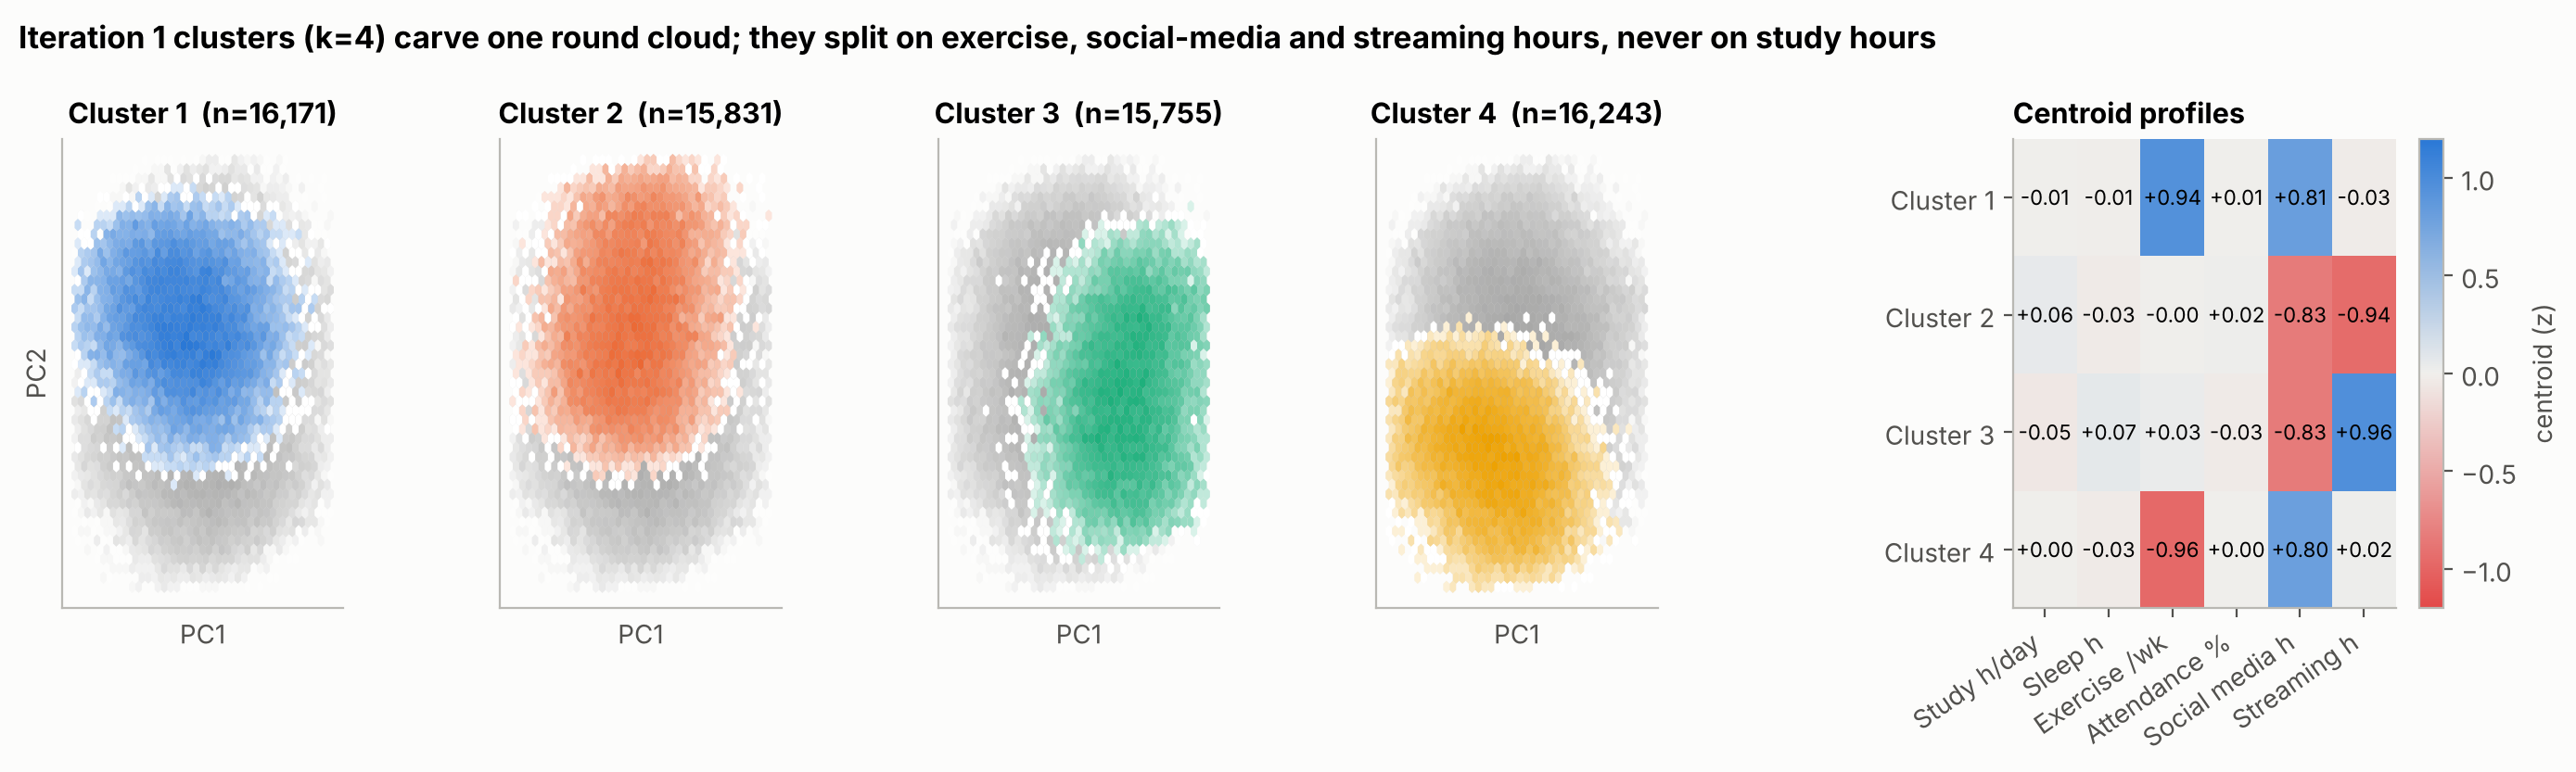
\includegraphics[width=\textwidth]{images/M1_fig03_cluster_map_raw.png}
  \caption{Iteration-1 clusters ($k=4$) on the first two principal components
  (which explain only 16.9\% and 16.7\% of variance). Each panel shows one
  cluster over the grey density of all students. The heatmap gives centroids in
  $z$-units: clusters differ by up to 1.9\,SD in exercise and streaming and
  1.6\,SD in social media, but by only 0.1\,SD in study hours and sleep.}
  \label{fig:m1-map1}
\end{figure}

Fig.~\ref{fig:m1-map1} shows K-means slicing one round cloud into four wedges.
The slices are defined by exercise, social media and streaming hours, two of
which have no relation to the score. Study hours, the habit most related to
the score, does not separate the clusters at all.

\begin{figure}[htbp]
  \centering
  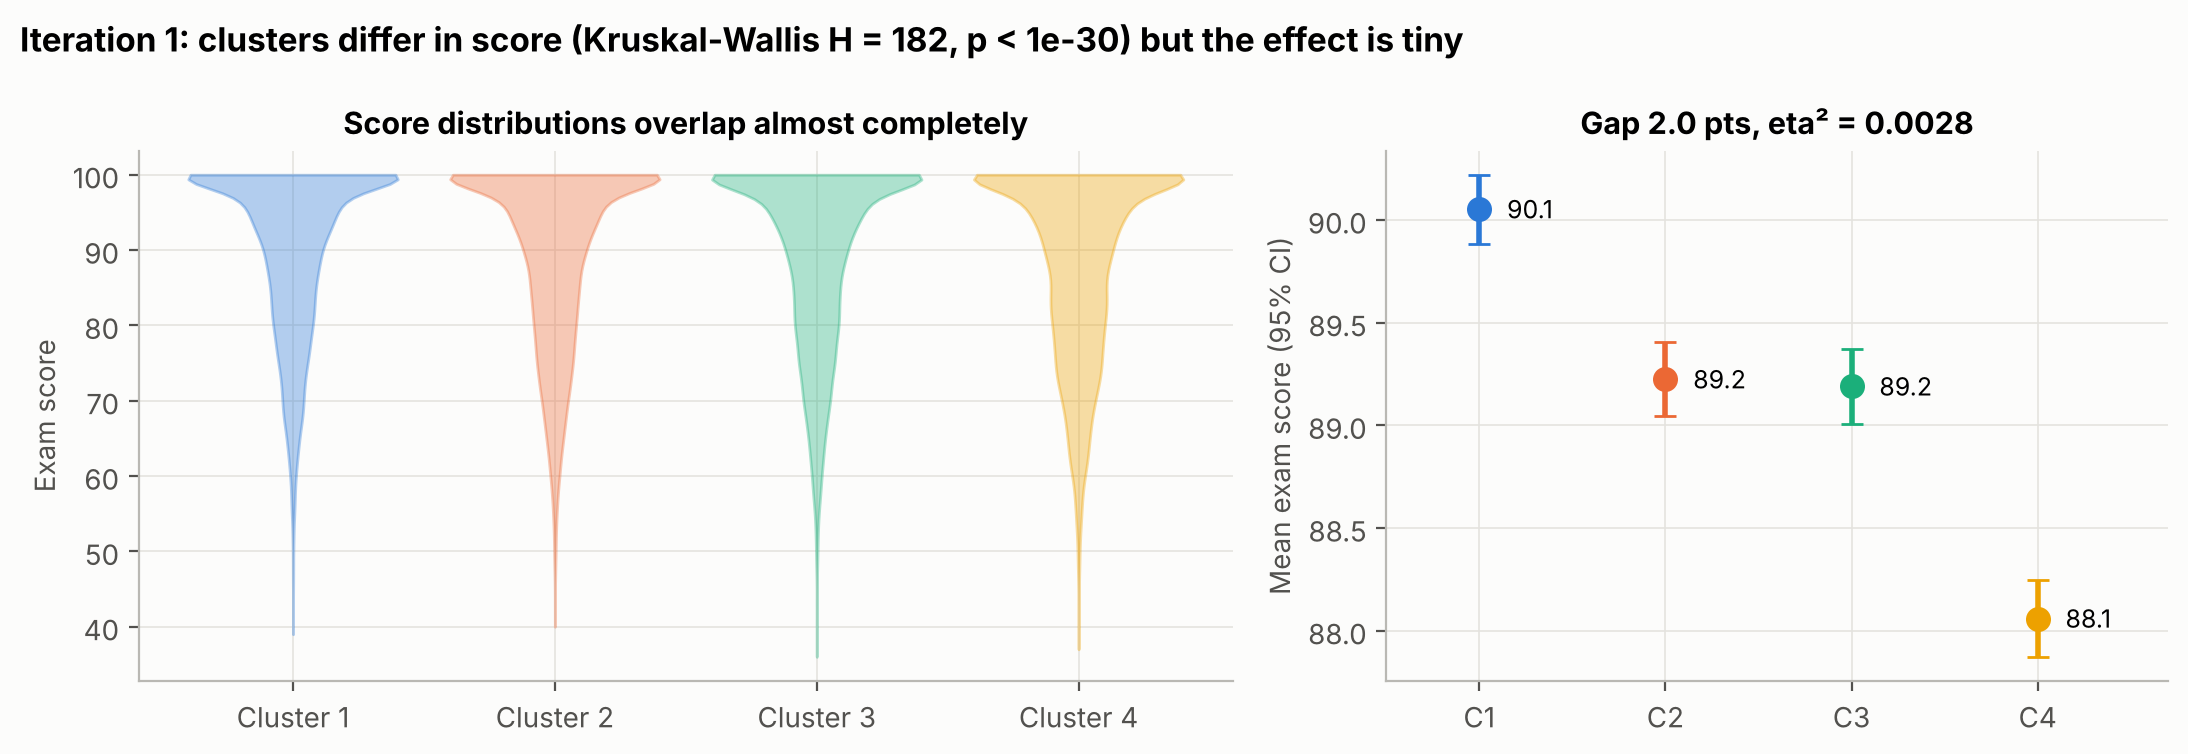
\includegraphics[width=\textwidth]{images/M1_fig04_score_by_cluster_raw.png}
  \caption{Exam score by iteration-1 cluster. The difference is statistically
  significant (Kruskal--Wallis $H=182$, $p=3\times10^{-39}$) but the effect
  size is negligible ($\eta^2_H=0.0028$): the best and worst clusters differ by
  2.0 points (90.1 vs.\ 88.1), and the distributions overlap almost entirely.}
  \label{fig:m1-score1}
\end{figure}

\begin{figure}[htbp]
  \centering
  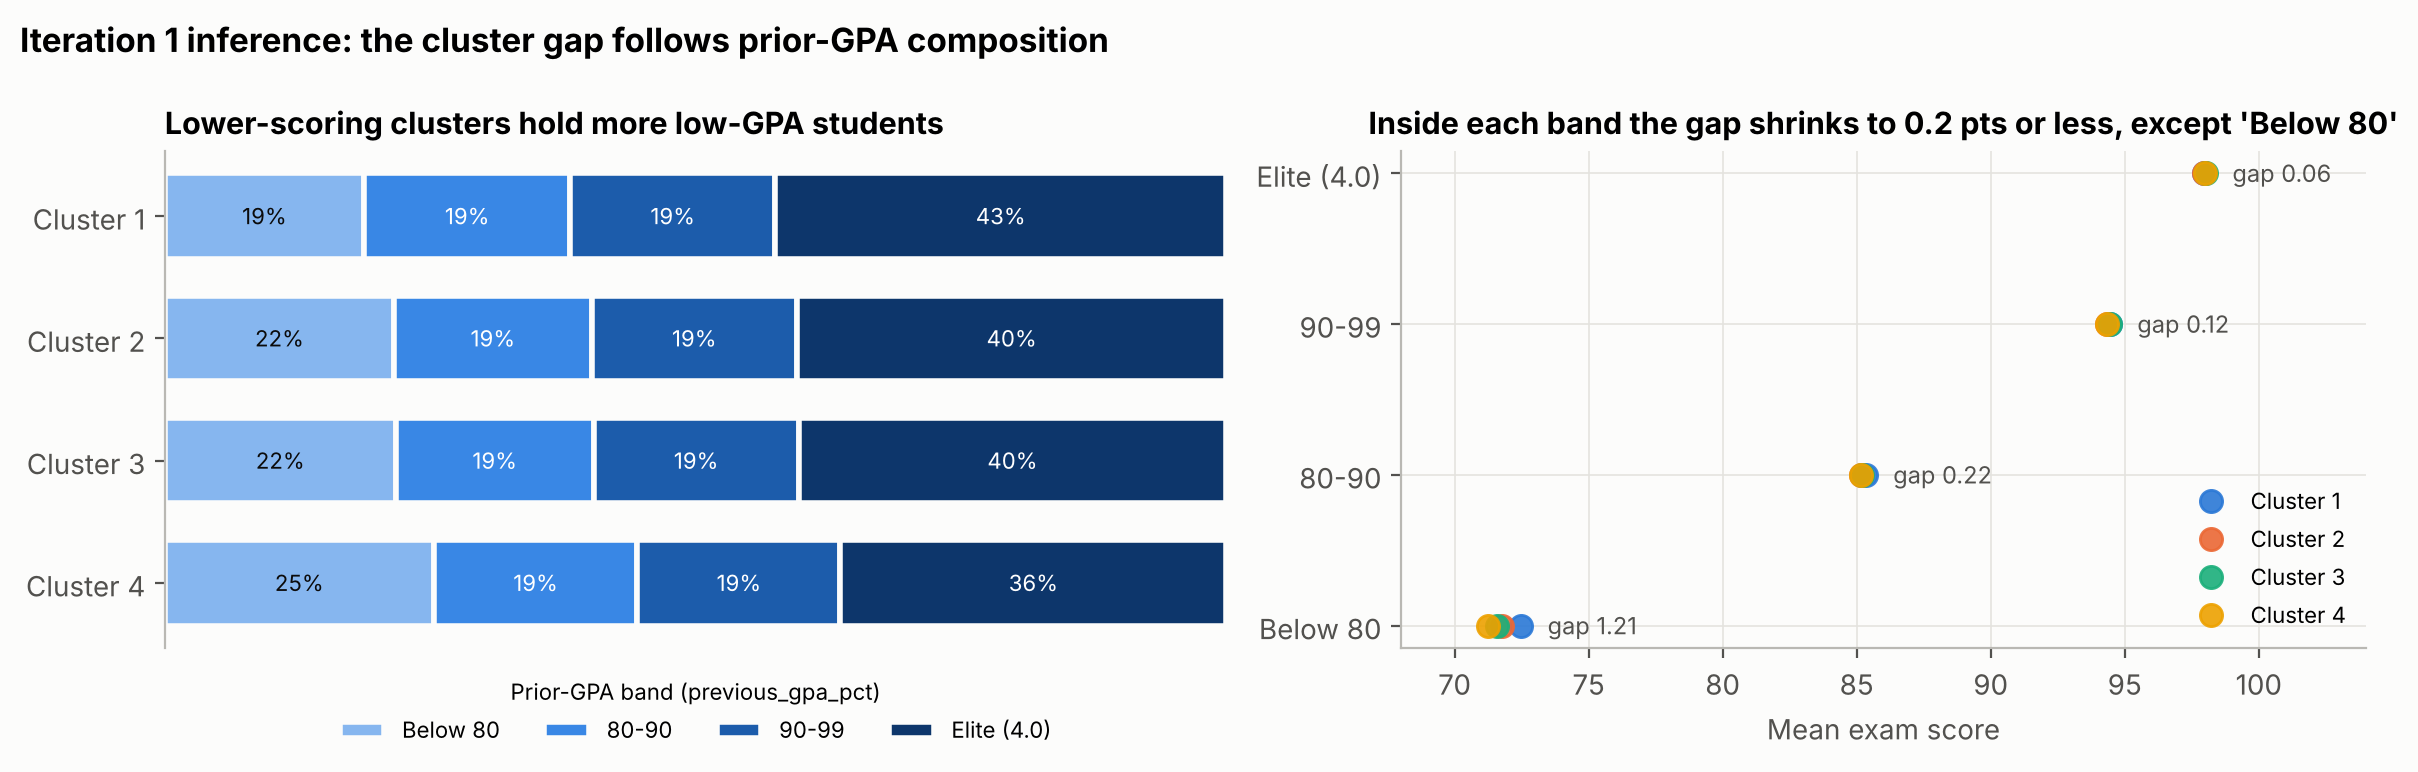
\includegraphics[width=\textwidth]{images/M1_fig05_gpa_confound_raw.png}
  \caption{Left: share of each cluster in each prior-GPA band. The lowest
  scoring cluster (C4) holds 25.3\% Below-80 students against 18.8\% for the
  highest (C1). Right: mean score per cluster inside each band. The cluster
  gap shrinks from 2.0 points to 0.06--0.22 points in the upper three bands;
  1.2 points remain in the Below-80 band.}
  \label{fig:m1-conf1}
\end{figure}

\paragraph{Knowledge K1.} Figs.~\ref{fig:m1-score1} and~\ref{fig:m1-conf1}
lead to three inferences:
\begin{enumerate}
  \item \textbf{The raw habit space has no natural clusters.} The silhouette
        equals that of shuffled data and partitions change with the random
        seed, so the iteration-1 clusters are arbitrary slices, not student
        types.
  \item \textbf{The slices follow the wrong variables.} Because the six
        habits are independent and equally weighted after scaling, K-means
        splits on whichever axes it happens to pick: here exercise, social
        media and streaming, not study hours. Raw leisure hours carry no signal;
        A1 (Appendix, Fig.~8) showed that the \emph{share} of screen time spent on
        leisure is what relates to performance.
  \item \textbf{The small score gap that exists is mostly prior GPA.} The
        clusters differ in their mix of prior-GPA bands, and inside a band the
        gap nearly disappears. The 1.2 points left in the Below-80 band need
        explaining: that band spans GPA 1.64--3.20, so students in it still
        differ a lot in prior attainment.
\end{enumerate}

% ---------------------------------------------------------------------------
\subsection{Feedback loop: transforming the data}

Each inference maps to one transformation of the data:

\begin{description}
  \item[T1 (feature space, from inferences 1--2).] Drop attendance, social media
        hours and streaming hours; add \texttt{leisure\_screen\_share}. The new
        space D2 holds four habits: study hours, sleep, exercise and leisure
        share. Leisure share correlates $r=-0.64$ with study hours, partly by
        construction (screen time includes study time). This dependence is
        what gives the space a real axis to cluster on: study-dominant versus
        leisure-dominant screen use.
  \item[T2 (target, from inference 3).] Replace the raw score with a
        \emph{GPA-adjusted score}: the student's score minus the mean score of
        all training students in the same prior-GPA bin (24 bins 0.1 GPA wide
        below 4.0, plus GPA exactly 4.0 as a 25th bin). Bin means are learned on the
        training split only and applied unchanged to the test split. These bin
        means alone explain $R^2=0.870$ of test-set score variance, so the
        adjusted score is the part of the exam that prior GPA does not predict
        (SD 4.2 points). Binning, rather than a straight-line fit, follows the
        curve near the ceiling without assuming its shape.
  \item[T3 (censoring).] 39.9\% of training students have GPA 4.0, and 53.6\%
        of those score exactly 100, so their adjusted score is capped. Every
        iteration-2 result is repeated with these students excluded.
\end{description}

% ---------------------------------------------------------------------------
\subsection{Iteration 2: clustering the refined habits}

\begin{figure}[htbp]
  \centering
  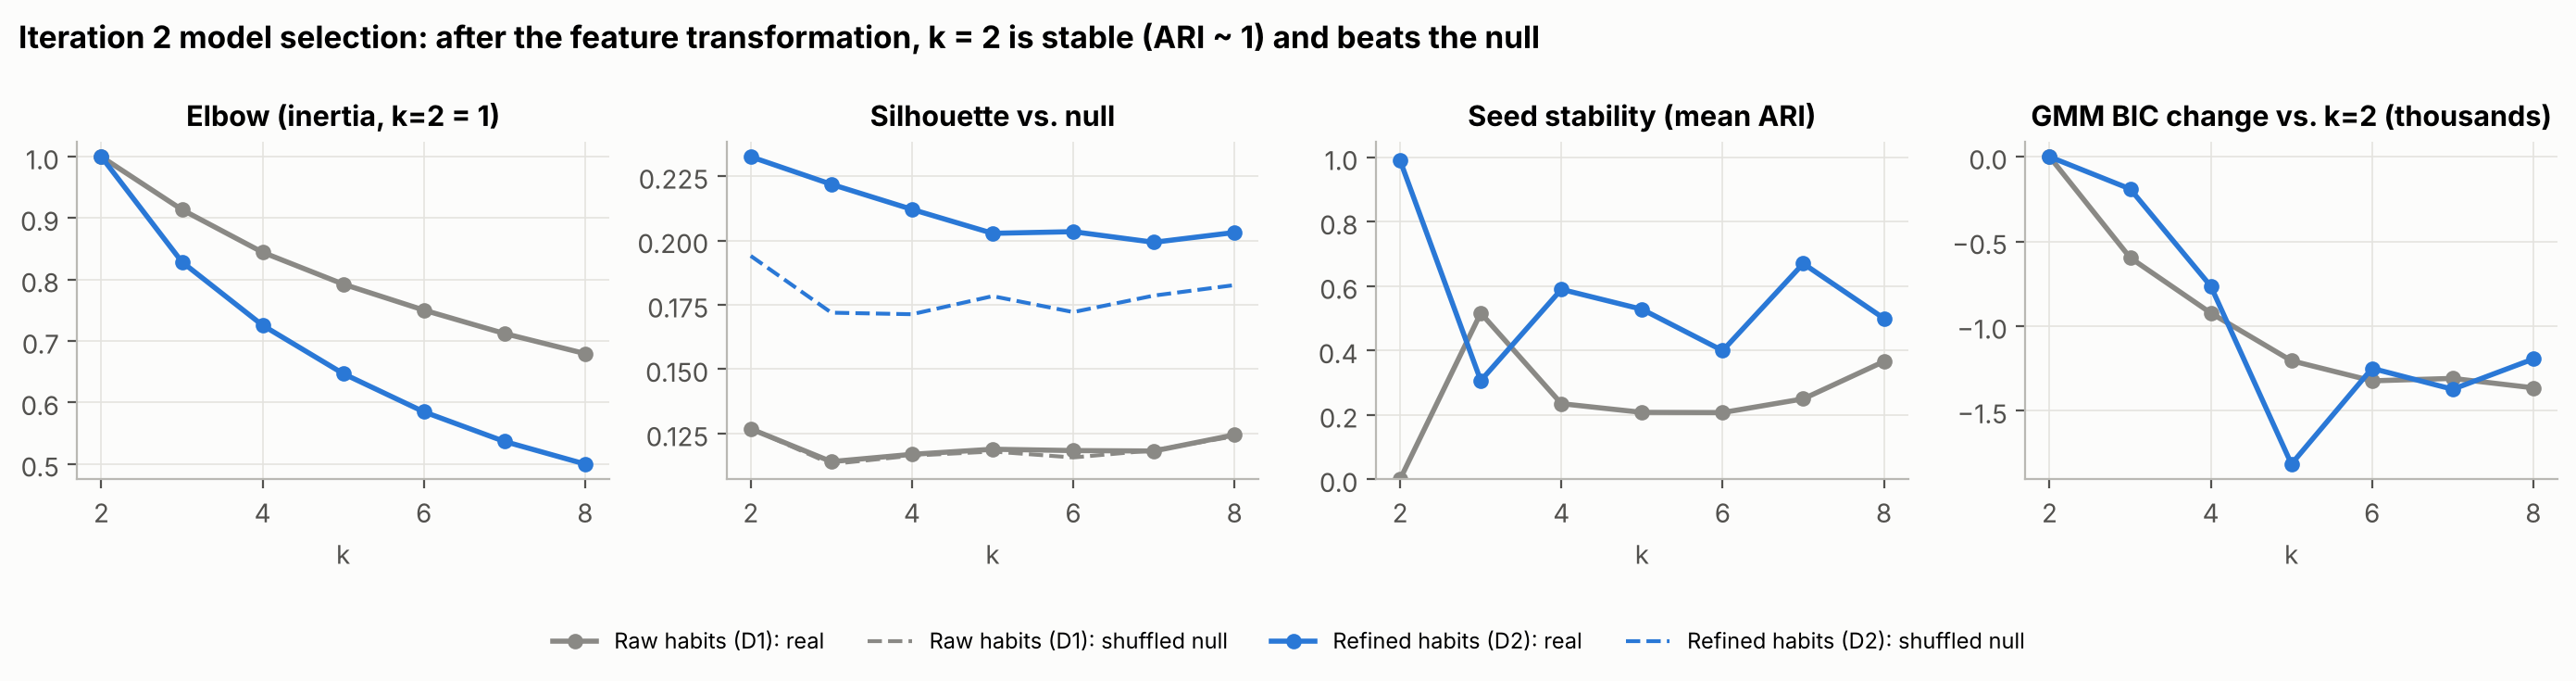
\includegraphics[width=\textwidth]{images/M1_fig06_k_selection_refined.png}
  \caption{Choosing $k$ on D2 (blue) against D1 (grey). At $k=2$ the refined
  space is now stable (ARI 0.99) and clearly above its null (silhouette 0.233
  vs.\ 0.194). GMM BIC is lowest at $k=5$, but that solution is not stable
  (ARI 0.53), so $k=2$ is used.}
  \label{fig:m1-k2}
\end{figure}

\paragraph{Model M2.} After T1, Fig.~\ref{fig:m1-k2} shows a real, repeatable
structure: six runs agree almost perfectly at $k=2$, and the silhouette beats
the shuffled null at every $k$. The pipeline selects $k$ automatically as the
most stable value. The Hopkins statistic rises to 0.88, but it is not used to
choose $k$: the leisure share and study hours fill only a triangular region
(Fig.~\ref{fig:m1-map2}), and a uniform reference sample drawn over the
bounding box inflates the statistic.

\begin{figure}[htbp]
  \centering
  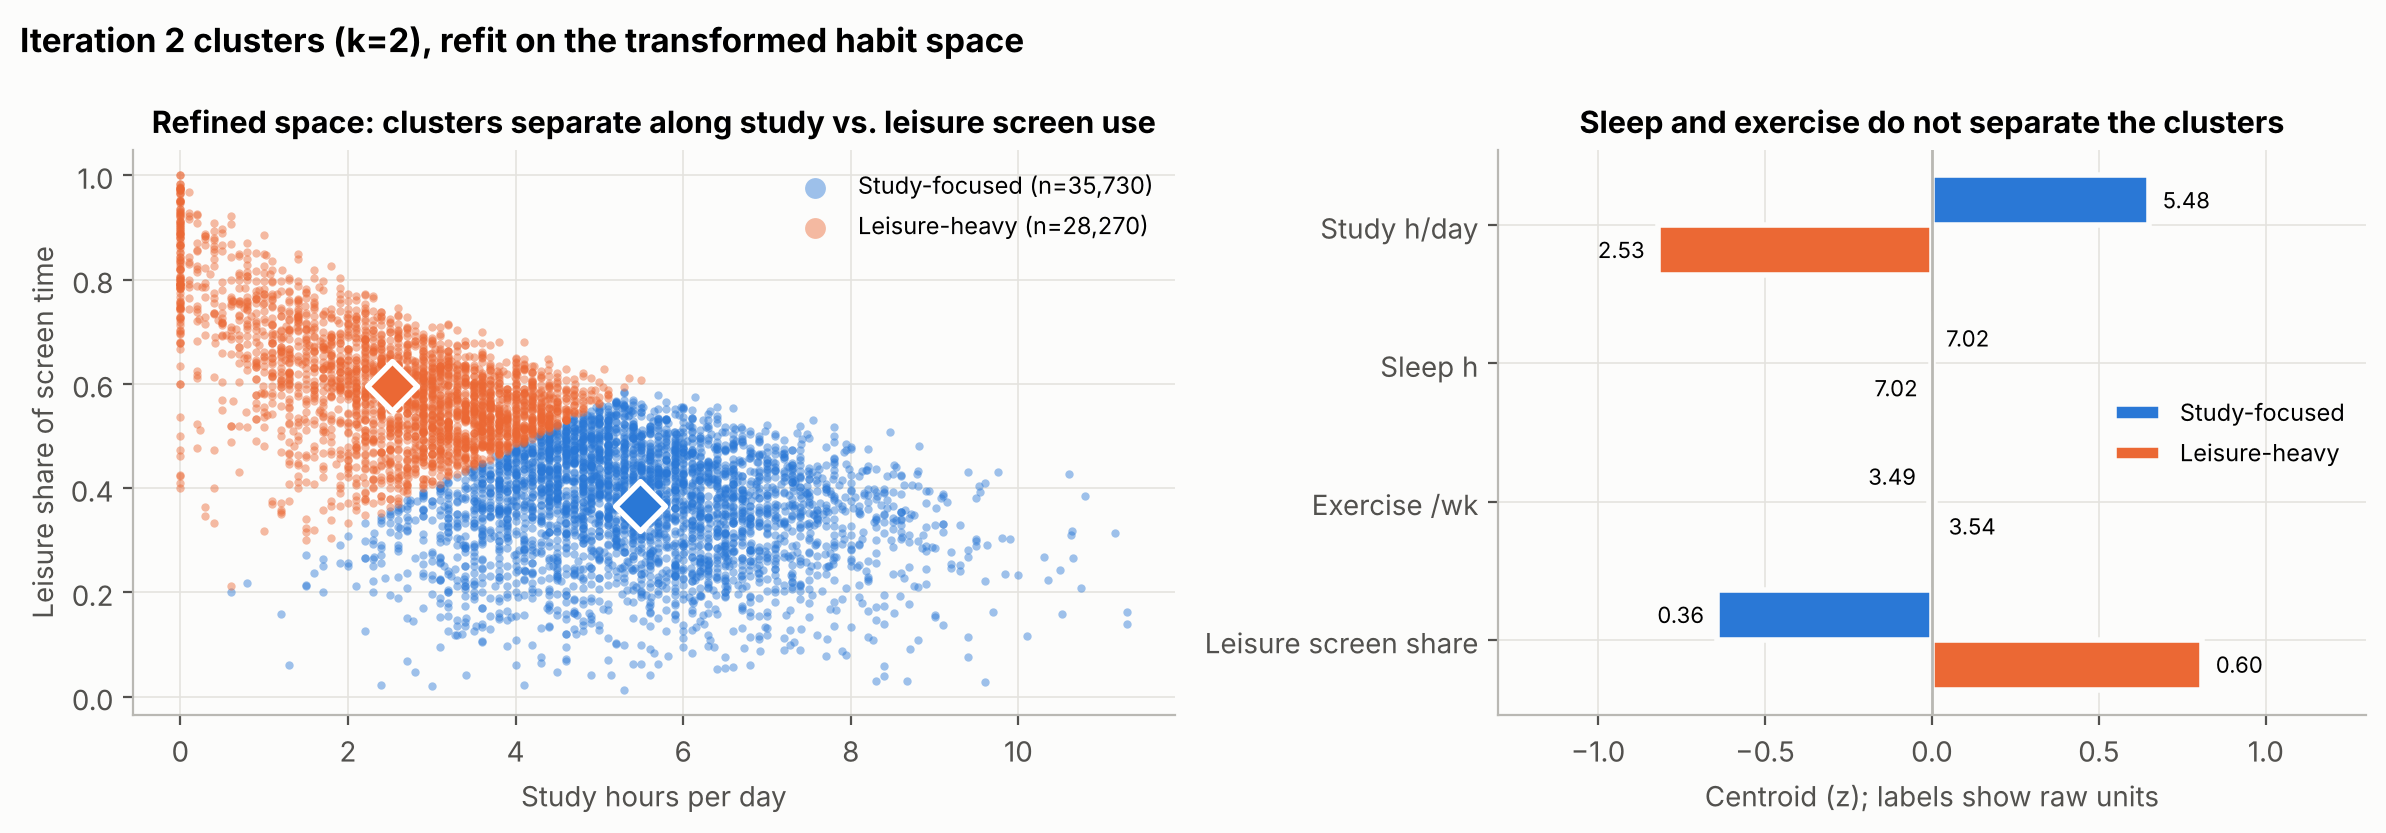
\includegraphics[width=\textwidth]{images/M1_fig07_cluster_map_refined.png}
  \caption{The two refined clusters. \emph{Study-focused} (35{,}730 training
  students) studies 5.5\,h/day with 37\% of screen time on leisure;
  \emph{Leisure-heavy} (28{,}270) studies 2.5\,h/day with 60\% on leisure.
  Sleep (7.0\,h both) and exercise (3.5 vs.\ 3.5 days) do not differ.
  Diamonds mark centroids.}
  \label{fig:m1-map2}
\end{figure}

\begin{figure}[htbp]
  \centering
  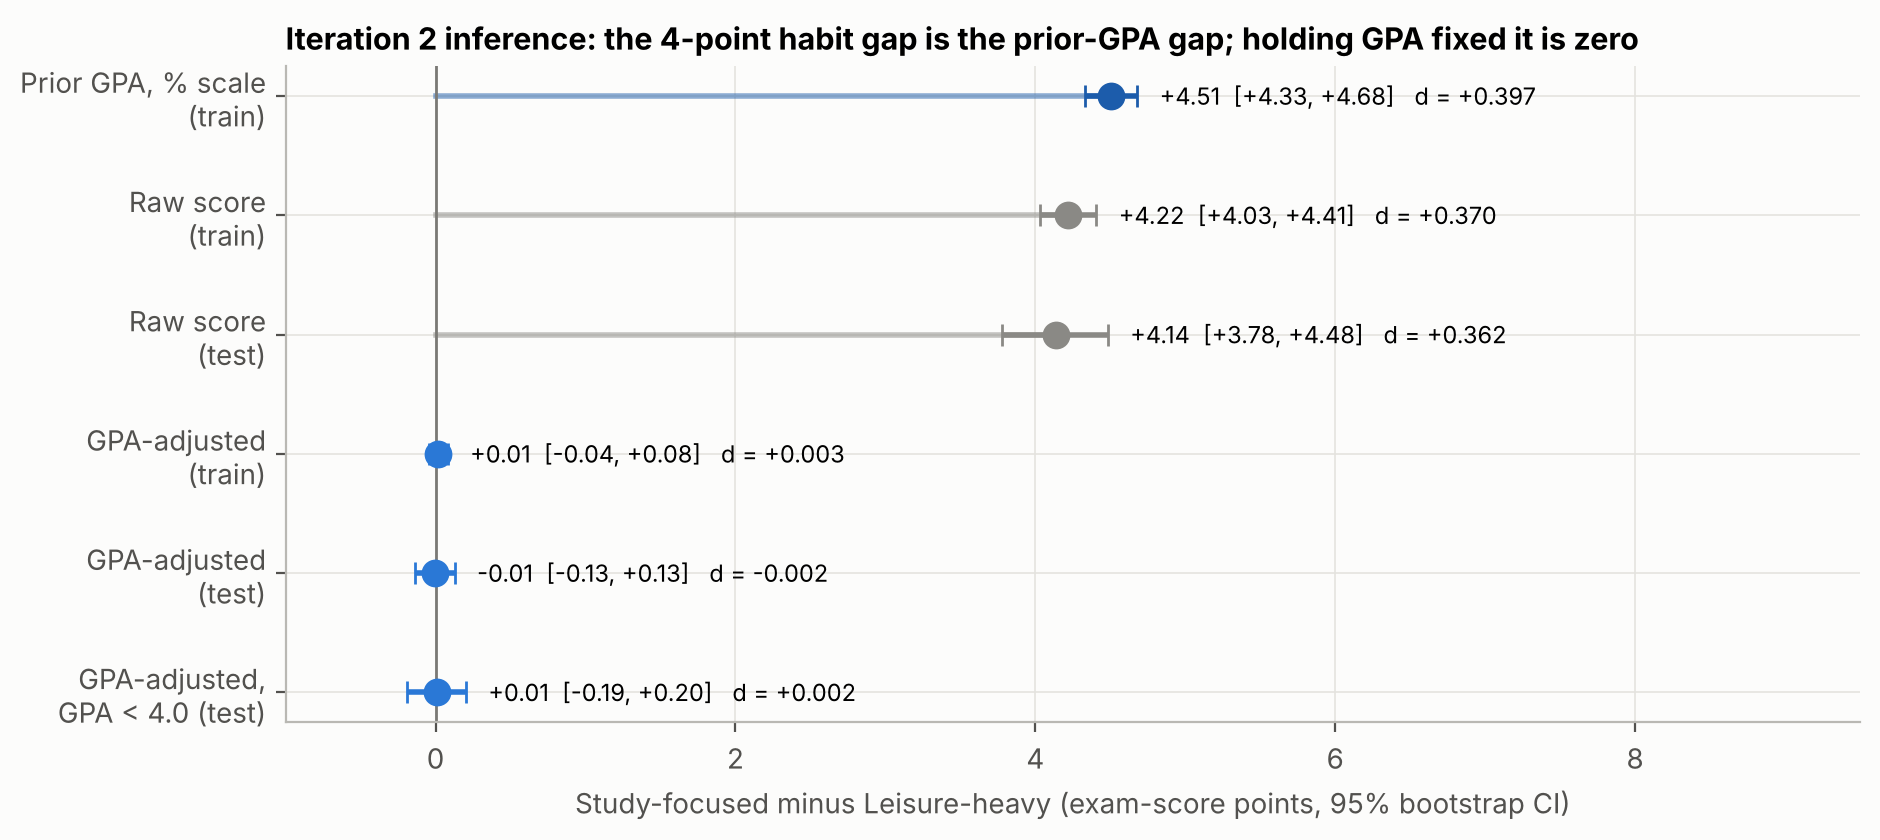
\includegraphics[width=\textwidth]{images/M1_fig08_raw_vs_adjusted_gap.png}
  \caption{Study-focused minus Leisure-heavy, in exam-score points, with 95\%
  bootstrap CIs. The raw gap is 4.2 points (test 4.1, $d=0.36$). The same
  clusters differ by 4.5 points in prior GPA on the percentage scale. On the
  GPA-adjusted score the gap is $+0.01$ (train) and $-0.01$ (test, CI
  $-0.13$ to $+0.13$, Welch $p=0.92$, $d=-0.002$), and stays at $+0.01$ with
  GPA-4.0 students removed.}
  \label{fig:m1-gap}
\end{figure}

\begin{figure}[htbp]
  \centering
  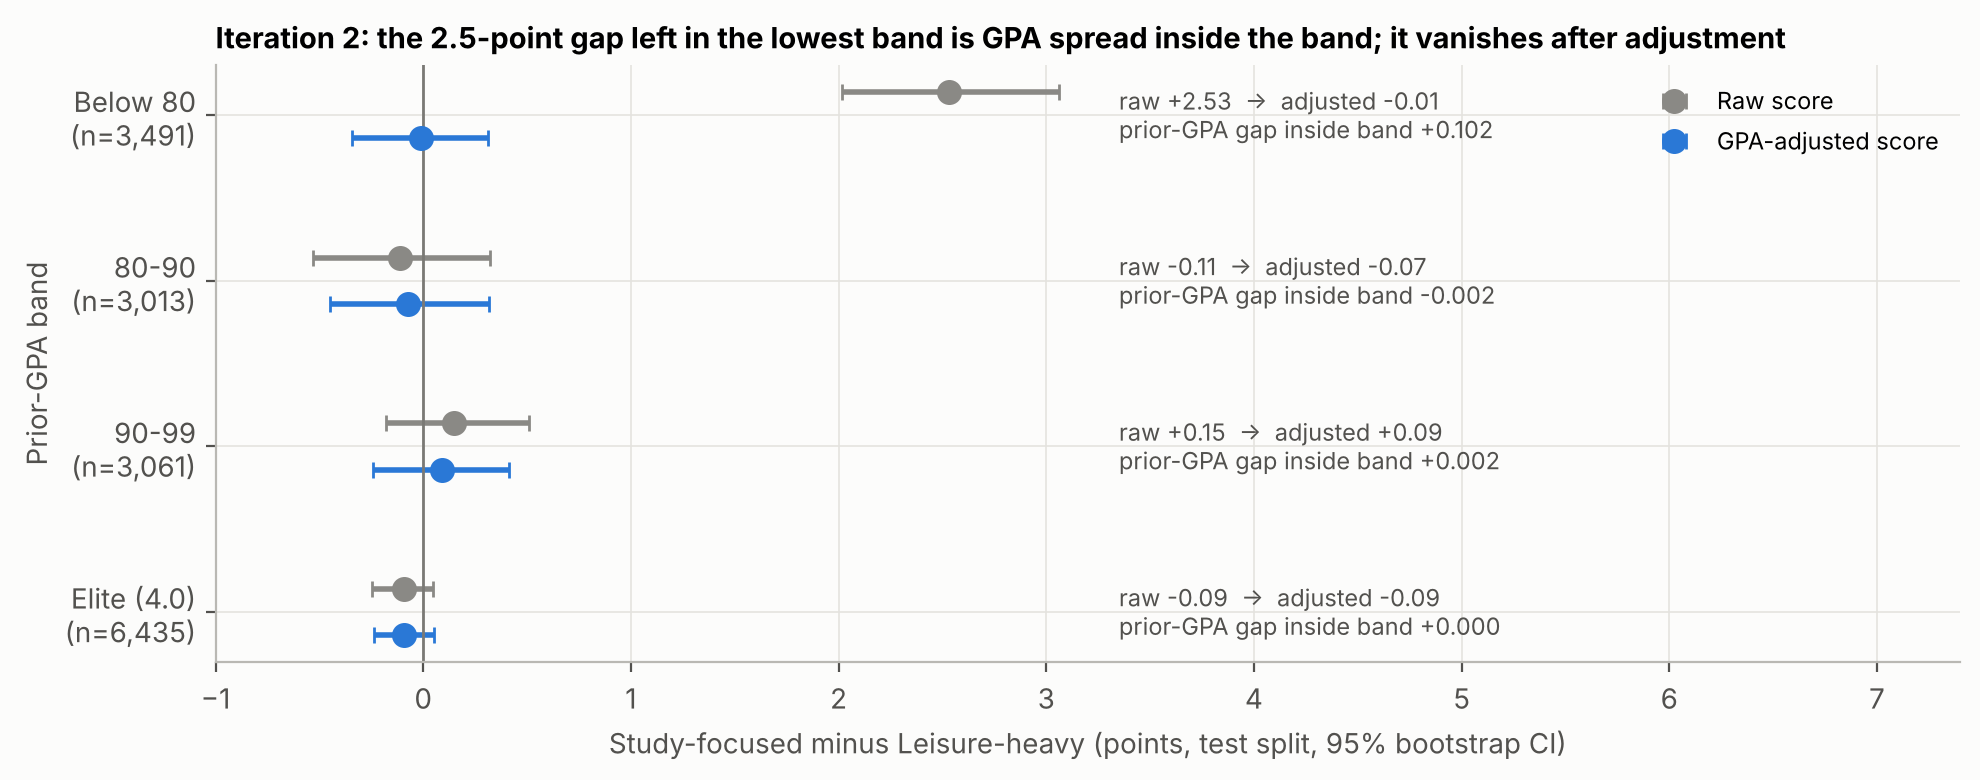
\includegraphics[width=\textwidth]{images/M1_fig09_within_band_refined.png}
  \caption{Gap per prior-GPA band on the test split, raw (grey) and adjusted
  (blue). The only raw gap left, 2.5 points in the Below-80 band, matches a
  0.10-point GPA difference between the clusters \emph{inside} that band. After
  adjustment it is $-0.01$ (CI $-0.34$ to $+0.31$). In the other bands both
  gaps are within $\pm0.15$.}
  \label{fig:m1-band}
\end{figure}

\begin{figure}[htbp]
  \centering
  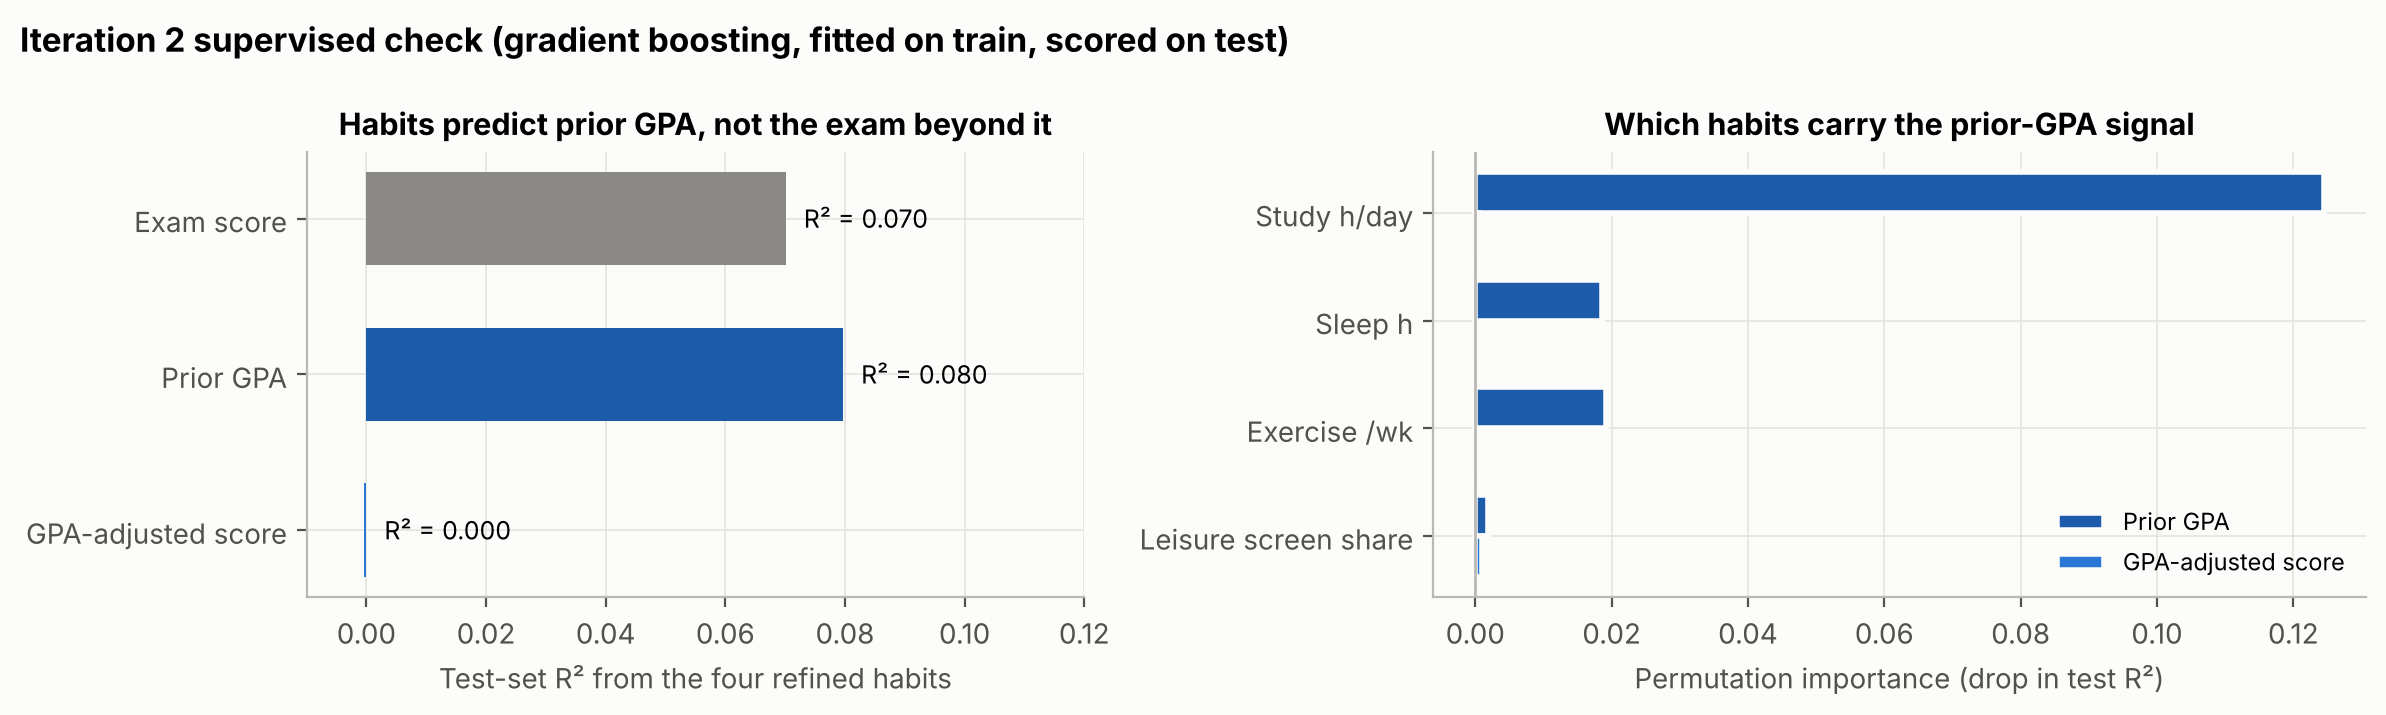
\includegraphics[width=\textwidth]{images/M1_fig10_supervised_check.png}
  \caption{Supervised check: gradient boosting fitted on the four refined
  habits (train) and scored on the test split. Habits explain $R^2=0.070$ of
  the exam score and 0.080 of prior GPA, but 0.000 of the GPA-adjusted score.
  Permutation importance shows study hours carries most of the prior-GPA
  signal; no habit carries any adjusted-score signal.}
  \label{fig:m1-sup}
\end{figure}

\paragraph{Knowledge K2.}
\begin{enumerate}
  \item \textbf{There is one stable habit profile split}, and it is about
        how students use screen time: study-focused versus leisure-heavy.
        Sleep and exercise do not form profiles of their own.
  \item \textbf{The profile's 4.2-point advantage is entirely its prior-GPA
        advantage.} Study-focused students arrive with a higher prior GPA; once
        GPA is held fixed, the gap is zero with a confidence interval narrower
        than $\pm0.13$ points, on unseen test data and with the ceiling group
        removed (Fig.~\ref{fig:m1-gap}).
  \item \textbf{Coarse bands hide confounding.} The Below-80 gap that survived
        banding in iteration~1 (Fig.~\ref{fig:m1-conf1}) is GPA variation
        inside the band (Fig.~\ref{fig:m1-band}). Any ``effect within the
        lowest band'' found with these four bands, including the one in A1
        (Appendix) Fig.~20, should be re-checked against the fine-grained adjustment.
  \item \textbf{Habits mark the trajectory, not the exam.} Habits predict prior
        GPA about as well as they predict the exam (Fig.~\ref{fig:m1-sup}).
        Prior GPA is measured before the exam and the habits are measured once,
        so this is a cross-sectional association: students with
        study-focused habits have been doing better for longer. The data cannot
        show that changing a habit would raise a score, and nothing in it
        suggests an exam-specific benefit.
\end{enumerate}

\paragraph{Reproducibility.} Running \texttt{preprocess\_a3.py} and then
\texttt{m1\_clustering\_workflow.py} (about one minute) regenerates every figure and number in this section. Cluster labels and the
adjusted score for all 80{,}000 students are saved for use in Tableau,
in \texttt{m1\_cluster\_assignments.csv.gz} under \texttt{Member1/outputs}.

\clearpage
% ---------------------------------------------------------------------------
% OWNER: Advaya Bhardwaj - what students feel (supervised classification).
% Follow TEAM_INSTRUCTIONS.md, Part B. Same structure as Section 4 (Tushaar):
% copy its style. Figures are already wired below: once your script saves
% images/M2_*.png with these names they appear automatically.
% Replace every \todo box; delete this comment block when done.
% ---------------------------------------------------------------------------
\section{Advaya Bhardwaj: Dropout Risk (Classification)}
\label{sec:m2}

\paragraph{Driving question.}
\todo{One paragraph. Suggested: A1 (Appendix, Fig.~21) found that the
dropout-risk flag is a hard rule on stress and motivation. Can a classifier
predict dropout risk, and once the rule's own inputs are removed, does anything
about a student still predict it?}

\paragraph{Method summary.}
\todo{One paragraph: logistic regression, decision tree, random forest
(scikit-learn~\cite{pedregosa2011}); class weights for the 2\% positive rate;
metrics are PR-AUC, ROC-AUC and F1 on the held-out test split (accuracy is
useless at 98\% negatives); permutation importance. Fit on train only.}

\teamfig{\textwidth}{images/M2_workflow_unrolled.png}{Member~2's workflow,
unrolled into two iterations with the \emph{Feedback loop} edge labelled.
\todoi{finish caption}}{fig:m2-workflow}

\todo{Add a task/rationale table like Table~\ref{tab:m1-tasks}: one row per
figure with stage, task verb and why that chart type.}

\subsection{Iteration 1: all features}

\teamfig{0.75\textwidth}{images/M2_fig01_rule_heatmap.png}{\todoi{Caption: dropout
rate for every stress $\times$ motivation cell on the training split.}}{fig:m2-rule}

\teamfig{\textwidth}{images/M2_fig02_iter1_pr_roc.png}{\todoi{Caption: PR and ROC
curves for the three models, test split. Quote PR-AUC per model.}}{fig:m2-pr1}

\teamfig{\textwidth}{images/M2_fig03_iter1_tree.png}{\todoi{Caption: depth-2 tree
and importances. The tree should split on stress $>8.05$ then
motivation $\le3.5$.}}{fig:m2-tree}

\paragraph{Knowledge K1.}
\todo{Numbered inferences. Expect: tree and forest reach PR-AUC 1.00;
logistic regression only about 0.88 because a straight boundary cannot draw an
AND-rectangle; the tree recovers the exact thresholds. Conclusion: the label is
a definition, so the models read it back (label leakage).}

\subsection{Feedback loop: transforming the data}
\todo{Describe T1: drop \texttt{stress\_level} and \texttt{motivation\_level}
(\texttt{exam\_anxiety\_score} is already removed in Section~\ref{sec:a3-prep});
keep class weights. Say why each change follows from K1.}

\subsection{Iteration 2: leak-free features}

\teamfig{\textwidth}{images/M2_fig04_iter2_pr_before_after.png}{\todoi{Caption:
PR curves before and after removing the rule variables, with the 2\% base
rate as a reference line.}}{fig:m2-pr2}

\teamfig{\textwidth}{images/M2_fig05_iter2_importance.png}{\todoi{Caption:
permutation importance of the leak-free model, test split.}}{fig:m2-imp}

\teamfig{\textwidth}{images/M2_fig06_proxy_check.png}{\todoi{Caption: dropout
rate by prior-GPA band and by mental-health rating.}}{fig:m2-proxy}

\paragraph{Knowledge K2.}
\todo{Numbered inferences. Expect: PR-AUC falls to about 0.04--0.08 (base rate
0.02) and ROC-AUC to about 0.70. Check which features carry the remaining
signal; a quick check found prior GPA alone gives ROC 0.67, because prior GPA
correlates $r=0.27$ with motivation, and mental health steps down at stress 7
(A1 Fig.~23). So what is left is mostly proxies for the two rule variables. Say
what this means: the flag measures how students feel, not what they do.}

\clearpage
% ---------------------------------------------------------------------------
% OWNER: Aman Kumar Lahoti - who students are (regression + statistics).
% Follow TEAM_INSTRUCTIONS.md, Part C. Same structure as Section 4 (Tushaar).
% Figures are wired below: once your script saves images/M3_*.png with these
% names they appear automatically. Replace every \todo box.
% ---------------------------------------------------------------------------
\section{Aman Kumar Lahoti: Exam Score (Regression and Statistical Tests)}
\label{sec:m3}

\paragraph{Driving question.}
\todo{One paragraph. Suggested: A1 (Appendix, Figs.~24--26) found tutoring to be
the one background lever (+2.8 points). How much of the exam score can be
modelled from all features, how does the 100-point ceiling distort that model,
and does tutoring survive once prior attainment is controlled?}

\paragraph{Method summary.}
\todo{One paragraph: OLS with HC3 robust errors (statsmodels~\cite{seabold2010})
and gradient boosting on the training split; test-set $R^2$/MAE; residual
diagnostics; then median (quantile) regression~\cite{koenker1978} and a
two-way ANOVA/ANCOVA for income $\times$ tutoring.}

\teamfig{\textwidth}{images/M3_workflow_unrolled.png}{Member~3's workflow,
unrolled into two iterations with the \emph{Feedback loop} edge labelled.
\todoi{finish caption}}{fig:m3-workflow}

\todo{Add a task/rationale table like Table~\ref{tab:m1-tasks}.}

\subsection{Iteration 1: all features, raw score}

\teamfig{\textwidth}{images/M3_fig01_iter1_fit.png}{\todoi{Caption: predicted vs.
actual (test) for OLS and gradient boosting; quote test $R^2$.}}{fig:m3-fit}

\teamfig{\textwidth}{images/M3_fig02_iter1_residuals.png}{\todoi{Caption: OLS
residual vs.\ fitted. The straight upper edge is the line
residual $=100-$fitted: the ceiling.}}{fig:m3-resid}

\teamfig{\textwidth}{images/M3_fig03_iter1_coefficients.png}{\todoi{Caption: OLS
coefficients with 95\% CIs (standardised).}}{fig:m3-coef}

\paragraph{Knowledge K1.}
\todo{Numbered inferences. Expect: OLS test $R^2\approx0.87$, essentially all
from prior GPA (slope about 23 points per GPA unit); every other coefficient is
near zero with $p>0.05$, including tutoring ($p\approx0.40$). About a quarter of
residuals sit exactly on the residual $=100-$fitted edge, and 40\% of students
share the single value GPA $=4.0$, so both ends of the model are censored. OLS
never predicts above 100 here; the censoring shows up as a residual edge, not as
impossible predictions.}

\subsection{Feedback loop: transforming the data}
\todo{T1: drop GPA $=4.0$ students (capped predictor; 40\% of rows).
T2: replace mean (OLS) with median regression, which is not moved by the
$\sim$7\% of the remaining students who score exactly 100.
T3: test tutoring with prior GPA as a covariate (ANCOVA). Say why each follows
from K1.}

\subsection{Iteration 2: censoring-aware models}

\teamfig{\textwidth}{images/M3_fig04_iter2_forest.png}{\todoi{Caption: coefficient
forest plot, median regression on GPA $<4.0$, with 95\% CIs.}}{fig:m3-forest}

\teamfig{\textwidth}{images/M3_fig05_iter2_tutoring.png}{\todoi{Caption: tutoring
gap by income band, raw vs.\ GPA-adjusted.}}{fig:m3-tutor}

\paragraph{Knowledge K2.}
\todo{Numbered inferences. Expect: in median regression on GPA $<4.0$, tutoring
$\approx0.00$ ($p\approx0.94$) and study hours $\approx0.00$; ANOVA raw shows
tutoring $p<10^{-100}$ with only a borderline income interaction ($p\approx0.05$); with prior GPA as covariate
tutoring $p\approx0.43$. Tutored students arrive with higher prior GPA (3.66
vs.\ 3.54). So A1's ``one real lever'' is also the prior-GPA confound. Discuss
time order: tutoring access and prior GPA are recorded together, so the data
cannot say which came first.}

\clearpage
% ---------------------------------------------------------------------------
% OWNERS: Advaya (writes) + Aman (checks). Tushaar's paragraph is DONE.
% ---------------------------------------------------------------------------
\section{Synthesis: One Story Across Three Strands}
\label{sec:synthesis}

\paragraph{From the clustering strand (Section~\ref{sec:m1}).}
The global K-means profiles differ by 4.15 exam points on the test set.
The higher-study profile contains more students who entered with a GPA of
4.0. Giving the two global clusters a common prior-GPA band distribution
reduces the difference to 0.51 points. Fitting new models in each band
yields a pooled contrast of 0.41 points for K-means and $-0.35$ for GMM.
The two models separate different habits in the lowest band. This limits
what the remaining contrast can tell us about a change in study time.

\todo{Add one paragraph each for the classification strand
(Section~\ref{sec:m2}) and the regression strand (Section~\ref{sec:m3}), in the
same style: what was found, the key number, what it means.}

\todo{Close by comparing the three strands against A1 Section~8 (Appendix).
Distinguish the strong association with prior GPA from the smaller remaining
differences: the habit contrast depends on the clustering method, the
tutoring interpretation needs adjustment for attainment, and the dropout
flag has an explicit definition. Use the final Member~2 and Member~3
results to establish which earlier readings are supported.}

% ---------------------------------------------------------------------------
% OWNER: Advaya. Short numbered list, one item per finding.
% ---------------------------------------------------------------------------
\section{Conclusions}
\label{sec:conclusions}

\begin{enumerate}
  \item Habit profiles exist only after feature transformation (one stable
        study-focused vs.\ leisure-heavy split), and their 4.2-point score gap
        is fully explained by prior GPA (adjusted gap $-0.01$, 95\% CI
        $\pm0.13$ on the test split). \emph{(Member~1)}
  \item \todo{Member~2's conclusion in one sentence.}
  \item \todo{Member~3's conclusion in one sentence.}
  \item \todo{One sentence on limitations: cross-sectional data, a synthetic-looking
        dataset with hard-coded rules, no causal claims.}
\end{enumerate}

% ---------------------------------------------------------------------------
% OWNERS: each member fills their own row. Tushaar's row is DONE.
% ---------------------------------------------------------------------------
\section{Author Contributions}
\label{sec:contrib}

\begin{table}[htbp]
  \centering\small
  \caption{Contribution of each team member.}
  \label{tab:contrib}
  \begin{tabular}{@{}p{3.2cm}p{12.3cm}@{}}
    \toprule
    Member & Contribution \\
    \midrule
    Kolipakula Sai Tushaar &
      Shared A3 preprocessing (\texttt{preprocess\_a3.py},
      \texttt{a3\_common.py}): validation, redundancy removal, leakage and
      ceiling flags, GPA bands, encoding, stratified split, shared palette.
      Member~1 strand (Section~\ref{sec:m1}): two-iteration clustering
      workflow in \texttt{Member1/m1\_clustering\_workflow.py}, ten figures,
      statistical tests and the gradient-boosting check. Workflow diagrams
      (Fig.~\ref{fig:master-workflow} and Fig.~\ref{fig:m1-workflow}), Sections
      \ref{sec:a3-prep}, \ref{sec:workflow} and \ref{sec:m1}, the report
      skeleton and team instructions. \\
    Advaya Bhardwaj & \todoi{Member~2 strand (classification of dropout risk),
      report assembly, Introduction, Synthesis, Conclusions.} \\
    Aman Kumar Lahoti & \todoi{Member~3 strand (regression and statistical
      tests), video demo and slides.} \\
    \bottomrule
  \end{tabular}
\end{table}

% ---------------------------------------------------------------------------
% References. Add yours as new \bibitem entries and cite them with \cite{key}.
% Entries used by Member 1 and the shared sections are DONE.
% ---------------------------------------------------------------------------
\begin{thebibliography}{99}

\bibitem{keim2008}
D.~Keim, G.~Andrienko, J.-D.~Fekete, C.~G\"{o}rg, J.~Kohlhammer and
G.~Melan\c{c}on, ``Visual analytics: Definition, process, and challenges,''
in A.~Kerren, J.~T.~Stasko, J.-D.~Fekete and C.~North (eds.),
\emph{Information Visualization}, LNCS vol.~4950, Springer, 2008,
pp.~154--175. doi:10.1007/978-3-540-70956-5\_7.

\bibitem{lloyd1982}
S.~P.~Lloyd, ``Least squares quantization in PCM,''
\emph{IEEE Transactions on Information Theory}, vol.~28, no.~2,
pp.~129--137, 1982.

\bibitem{rousseeuw1987}
P.~J.~Rousseeuw, ``Silhouettes: A graphical aid to the interpretation and
validation of cluster analysis,'' \emph{Journal of Computational and Applied
Mathematics}, vol.~20, pp.~53--65, 1987.

\bibitem{dempster1977}
A.~P.~Dempster, N.~M.~Laird and D.~B.~Rubin, \emph{Maximum likelihood from
incomplete data via the EM algorithm}, Journal of the Royal Statistical
Society, Series B, vol.~39, no.~1, pp.~1--22, 1977.
\href{https://doi.org/10.1111/j.2517-6161.1977.tb01600.x}{doi:10.1111/j.2517-6161.1977.tb01600.x}.

\bibitem{holm1979}
S.~Holm, \emph{A simple sequentially rejective multiple test procedure},
Scandinavian Journal of Statistics, vol.~6, no.~2, pp.~65--70,
1979. \href{https://www.jstor.org/stable/4615733}{JSTOR 4615733}.

\bibitem{hubert1985}
L.~Hubert and P.~Arabie, ``Comparing partitions,''
\emph{Journal of Classification}, vol.~2, no.~1, pp.~193--218, 1985.

\bibitem{hopkins1954}
B.~Hopkins and J.~G.~Skellam, ``A new method for determining the type of
distribution of plant individuals,'' \emph{Annals of Botany}, vol.~18, no.~2,
pp.~213--227, 1954.

\bibitem{kruskal1952}
W.~H.~Kruskal and W.~A.~Wallis, ``Use of ranks in one-criterion variance
analysis,'' \emph{Journal of the American Statistical Association}, vol.~47,
no.~260, pp.~583--621, 1952.

\bibitem{welch1947}
B.~L.~Welch, ``The generalization of `Student's' problem when several
different population variances are involved,'' \emph{Biometrika}, vol.~34,
pp.~28--35, 1947.

\bibitem{mann1947}
H.~B.~Mann and D.~R.~Whitney, ``On a test of whether one of two random
variables is stochastically larger than the other,'' \emph{Annals of
Mathematical Statistics}, vol.~18, no.~1, pp.~50--60, 1947.

\bibitem{cohen1988}
J.~Cohen, \emph{Statistical Power Analysis for the Behavioral Sciences},
2nd ed., Lawrence Erlbaum Associates, 1988.

\bibitem{efron1993}
B.~Efron and R.~J.~Tibshirani, \emph{An Introduction to the Bootstrap},
Chapman \& Hall, 1993.

\bibitem{friedman2001}
J.~H.~Friedman, ``Greedy function approximation: A gradient boosting
machine,'' \emph{Annals of Statistics}, vol.~29, no.~5, pp.~1189--1232, 2001.

\bibitem{breiman2001}
L.~Breiman, ``Random forests,'' \emph{Machine Learning}, vol.~45, no.~1,
pp.~5--32, 2001.

\bibitem{pedregosa2011}
F.~Pedregosa et~al., ``Scikit-learn: Machine learning in Python,''
\emph{Journal of Machine Learning Research}, vol.~12, pp.~2825--2830, 2011.

\bibitem{seabold2010}
S.~Seabold and J.~Perktold, ``Statsmodels: Econometric and statistical
modeling with Python,'' in \emph{Proceedings of the 9th Python in Science
Conference}, 2010, pp.~92--96.

\bibitem{koenker1978}
R.~Koenker and G.~Bassett, ``Regression quantiles,'' \emph{Econometrica},
vol.~46, no.~1, pp.~33--50, 1978.

\end{thebibliography}


\clearpage
\appendix
\section{Appendix: A1 Report}
\label{app:a1}
The A1 report is included for completeness, as the brief requires. It is not
assessed as part of A3.
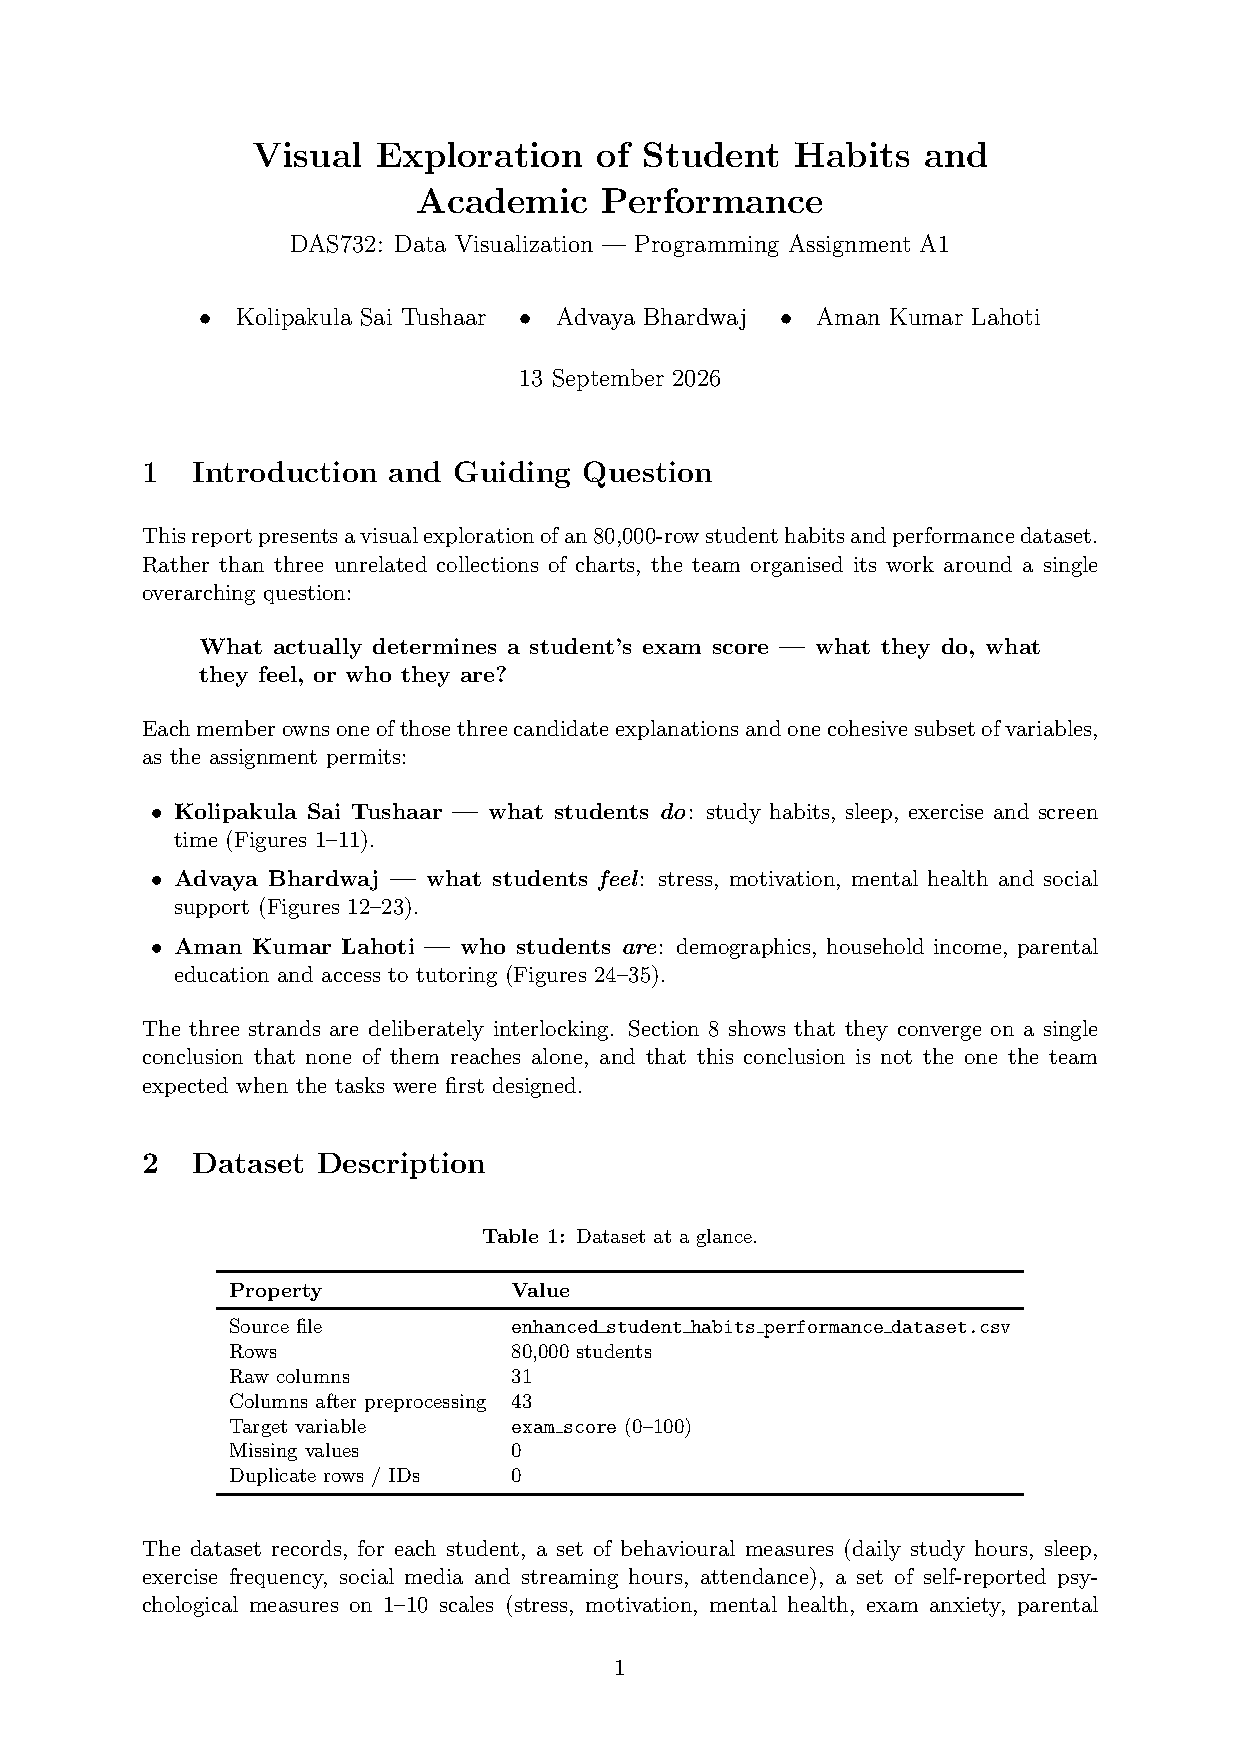
\includepdf[pages=-,scale=0.92,pagecommand={\thispagestyle{plain}}]{../reference/DV_Assignment1_report.pdf}
\end{document}
